\documentclass[]{article}
\usepackage{lmodern}
\usepackage{truncate}
\usepackage{caption}
\usepackage{tocloft}
\usepackage{amssymb,amsmath}
\usepackage{ifxetex,ifluatex}
\usepackage{fixltx2e} % provides \textsubscript

\usepackage{longtable}
\usepackage{graphicx}
\usepackage[table]{xcolor}

\makeatletter
\def\maxwidth{\ifdim\Gin@nat@width>\linewidth\linewidth\else\Gin@nat@width\fi}
\def\maxheight{\ifdim\Gin@nat@height>\textheight\textheight\else\Gin@nat@height\fi}
\makeatother

% Scale images if necessary, so that they will not overflow the page
% margins by default, and it is still possible to overwrite the defaults
% using explicit options in \includegraphics[width, height, ...]{}
\setkeys{Gin}{width=\maxwidth,height=\maxheight,keepaspectratio}
\ifxetex
  \usepackage[setpagesize=false, % page size defined by xetex
              unicode=false, % unicode breaks when used with xetex
              xetex]{hyperref}
\else
  \usepackage[unicode=true]{hyperref}
\fi
\hypersetup{breaklinks=true,
            bookmarks=true,
            pdfauthor={M.D.~Catchen},
            pdftitle={Dissertation Prospectus},
            colorlinks=true,
            citecolor=blue,
            urlcolor=blue,
            linkcolor=magenta,
            pdfborder={0 0 0}}
\urlstyle{same}  % don't use monospace font for urls


\setlength{\parindent}{0pt}
\setlength{\parskip}{6pt plus 2pt minus 1pt}
\setlength{\emergencystretch}{3em}  % prevent overfull lines
\setcounter{secnumdepth}{0}

\title{Dissertation Prospectus}
\author{M.D.~Catchen}
\date{}

% Table of contents formatting
\setcounter{secnumdepth}{3}
\addtocontents{toc}{\setcounter{tocdepth}{2}}

\usepackage[left=1.5in,right=1.5in]{geometry}
\setlength{\parskip}{12pt}

% Headers and page numbering
\usepackage{fancyhdr}
\pagestyle{fancy}
\lhead{  \nouppercase  \leftmark}
\rhead{\thepage}
\cfoot{}

% Table package
\usepackage{ctable}% http://ctan.org/pkg/ctable

\usepackage{titling}
\pretitle{\begin{flushleft}\Large\bfseries}
\posttitle{\end{flushleft}}
\preauthor{\begin{flushleft}\large}
\postauthor{\end{flushleft}}
\predate{\begin{flushleft}\large}
\postdate{\end{flushleft}}

\usepackage{float}
\floatplacement{figure}{h}

\usepackage{morefloats}
% or use \extrafloats{100}
% add some \clearpage

\usepackage{sectsty}
\usepackage[normalem]{ulem}
\sectionfont{\rmfamily\bfseries\large}
\subsectionfont{\rmfamily\bfseries\centering\upshape\normalsize}
\subsubsectionfont{\rmfamily\itshape\centering\normalsize}

% % Chapter header
\usepackage{titlesec, blindtext, color}
\definecolor{gray75}{gray}{0.75}
\newcommand{\hsp}{\hspace{20pt}}


\titleformat{\chapter}[display]
{\normalfont\Large\bfseries}{Chapter\ \thechapter}{0em}{
\vspace{-1em}
}
[
\vspace{-2.8em}
]

\titlespacing*{\chapter}{0pt}{0pt}{40pt}

% FONTS
\fontsize 12

% CODE BLOCKS
\usepackage[utf8]{inputenc}
\usepackage{listings}
\usepackage{color}
\DeclareMathSizes{12}{13}{7}{7}


\usepackage{lineno}

% Set figure legends and captions to be smaller sized sans serif font
\usepackage[font={footnotesize,sf}]{caption}
\usepackage{siunitx}

\usepackage{setspace}
\linespread{1.2}
\raggedbottom

\usepackage{hyperref}

\usepackage[square, numbers]{natbib}
\bibliographystyle{unsrtnat}

% Tables

\usepackage{booktabs}
\usepackage{threeparttable}
\usepackage{array}


\begin{document}
\maketitle
\begin{abstract}
Forecasting the future of Earth's ecosystems under Anthropogenic change is no small task.
Robust prediction has long evaded ecological processes due to their inherently complex, stochastic, and emergent nature.
Many disciplines that deal with similarly complex phenomena have benefited from using simulation models as tools for both forecasting and inference, but in this realm, ecology has been a slow adopter.
There is much to be gained in biodiversity science from the further adoption of these methods as regular.
Here, we outline the potential for simulation models in metacommunity ecology, both for answering fundamental questions about the structure of ecological communities, but also for application in the management of real systems facing climatic and land-use change.
We discuss how simulation models can be used to make predictions with real data, and then
describe a process-based model of metacommunity dynamics (based around \citep{vellend_conceptual_2010, poisot_beyond_2015, thompson_process-based_2020}), and detail how we'll implement this model as software that is modular and can be used to answer a variety of questions about metacommunity dynamics, both in the ``virtual laboratory" case \citep{railsback_agent-based_2011}, as well in empirical systems.
At the moment, there do not exist software tools that exist explicitly for the purpose of forecasting community structure under a given model of future climate and land use, and building and applying this type of software is the primary goal of the dissertation.
We then conclude by outlining the structure of the proposed chapters.
\end{abstract}

\pagebreak

{
\singlespacing
\small

\begin{quote}
\begin{flushright}
\textit{La guêpe et l'orchidée font rhizome, en tant que hétérogènes}\end{flushright}


\begin{flushright}
\text{Deleuze and Guattari}, \textit{Plateau mille} \end{flushright}

\end{quote}

\vspace{10mm}

\begin{quote}
    \begin{flushright}
    \textit{Given the nature of all this new shit, you know, I-I... this could be a lot more, uh, uh, complex, I mean, it's not just, it might not be just such a simple... uh, you know?} \end{flushright}

    \begin{flushright}
        \text{Joel \& Ethan Coen}, \textit{The Big Lebowski } \text{(1997)}
    \end{flushright}
\end{quote}
}

\vspace{30mm}

{
\hypersetup{linkcolor=black}
\setcounter{tocdepth}{3}
\normalfont
\tableofcontents
}
\pagebreak



% ________________________________________________________________________
%
%       CHAPTER 1
%
%       introduction

% ________________________________________________________________________
\hypertarget{introduction}{%
\section{Introduction}\label{introduction}}

When Edmond Halley predicted his now eponymous comet's return to Earth 76 years in advance, it would have made sense to bet against him---after all, humans had been trying to forecast the appearance of comets and meteors for millennia, with little success. But Halley was the first to predict a comet's trajectory using the recently developed methods of Newtonian and Keplerian mechanics.
Halley conjectured that past observations of ``different" comets, each appearing roughly 76 years after the previous, were in fact the same object, and that the variability in the comet's period was attributable to the variable gravitational influence of Jupiter and Saturn.
His computations enabled him to successfully predict the comet's eventual return to Earth in 1758, and his prediction provided one of the foundational pieces of evidence for Kepler and Newton's models. Halley's success also further embedded methodological reductionism as the principal method of scientific discovery.
Since Halley's time, the problem solving strategy of starting with the simplest case and gradually building toward a higher fidelity representation of the system has become a ubiquitous tool across the sciences \cite{polya_how_2009}.
There are good reasons for this---the limitations of analytical mathematics made high-dimensional representations of a system intractable, and therefore reducing a model to as few measurable values as possible was necessary to interface with the quantitative tools of the time. Of course, in reality every natural system is complex.
The motion of matter is subject to the ever-changing pairwise gravitational forces of all other matter in existence, and yet Halley was successful in predicting the dynamics of his comet by considering only a small subset of those interactions.
Not only that, but Newtonian mechanics adds the additional abstraction of representing the state of each object with only two values, position and momentum. Surely if one were to study the distribution of matter within the Sun, describing it as a single point at its center would seem overzealous. Yet, this abstraction did not invalidate Halley's model because the effects of internal heterogeneity are practically immeasurable on the scale of the entire system \cite{levins_dialectical_1987}.

 In ecology (and the biological sciences in general) we are not so lucky---the properties of the systems we study are emergent, and do not exist when we reduce a system down to its simplest form.
For example, consider the Lotka-Volterra model.
Much like the model of Newtonian gravity Halley applied to his comet, LV is written in the
language of coupled differential equations\footnote{The reality is computing the gravitational dynamics of more than two bodies of comparable mass is, much like ecological modeling, tough. Halley's work avoided the infamous n-body problem, but modern astrodynamicists use simulation models for many of the same reasons we advocate their use in ecology, coming up in the main text.}.
The characteristic feature of the two-species LV model are its boom-and-bust limit cycles, and this qualitative behavior is observed in many systems.
In controlled settings, LV can make fairly good predictions about the abundances of predator and prey \cite{varon_bacterial_1978, fussmann_crossing_2000}, but in complex ecosystems, the \(n\)-species generalized LV model doesn't succeed at making predictions with much accuracy \cite{momeni_lotka-volterra_2017}, 76 years out or otherwise.
This is not to say LV is not interesting and worthy of study in its own right---it is what Okubo (1972) calls a ``toy model" \cite{okubo_diffusion_2001}---an intentional oversimplification that can explore the fundamental mechanisms driving real systems.
However, for the purposes of forecasting, there is at least enough influence on the abundance of each species from the combined factors of environmental and demographic stochasticity, trait-matching in interactions, spatial heterogeneity, and so on, that LV isn't suited for applications in conservation or management of real systems.
Trophic interactions between pairs of species are the building blocks of ecological communities, and yet the properties of communities cannot be understood simply by generalizing LV to larger systems, as there are latent processes, both deterministic and stochastic, structuring communities that are only apparent outside the scope of any particular interaction between predator and prey. This is the essence of what make any system \emph{complex}.


Ecological systems have long evaded effective prediction because there is internal heterogeneity at all scales of biological organization \citep{levins_dialectical_1987,levin_problem_1992}, and the effects of this heterogeneity propagate across scales.
In community ecology, it seems the atomic level of organization is naturally the individual of any given species.
Yet, adopting the Platonic form ``individual" with property ``species" neglects the immense variability in the biological processes that compose any given individual, and the variability of the individuals that compose a species.
Certainly this abstraction would cause consternation from the behavioral ecologists down the hall, to the cell biologists studying gene expression, to the biochemists in the next building, etc.
This is not to say that we should build ecological models starting from the building blocks of particle physics in order to encapsulate the heterogeneity across the spectrum of levels of biological organization \citep{levin_problem_1992}, but instead we must be cognizant of what our models treat as internally homogeneous---a false premise in biological systems.
In \emph{The Dialectical Biologist}, Lewontin and Levins write:

\begin{quote}
A space capsule could not land on the moon without Newtonian
abstractions, nor could it land with them alone. The problem for science
is to understand the proper domain of explanation of each abstraction
rather than become its prisoner. \citep{levin_problem_1992}
\end{quote}

\clearpage
Widely across fields, computer simulation models have upended the methods of science, precisely because they enable us to explore the
``proper domain of explanation of each abstraction" with more care, and often less required expertise\footnote{In the sense that computer software can often be implemented by a person whose is a non-expert in the methods of the software, but is using it for an applied purpose, see much of bioinformatics as an example.} than the tools of analytical math.
The modular nature of software means any conceptual object used in a simulation model can be represented in as much fidelity as the author chooses.
One can implement the LV model (without any in-depth knowledge of how to solve differential equations, in fact) in 30 lines of code, or create the most convoluted individual-based model imaginable---it then becomes within the author's purview to define the ``proper domain of explanation of each abstraction."

Using simulation models, we contest, we can now explore the complex processes that produce the astounding biodiversity we see on Earth in far more detail, and with greater respect toward their complexity than canned statistical models.
Further, these tools have strong potential as we attempt to predict the consequences of the dramatic influence humans have on our planet and the life to which it is a unique home.
Simulation models have now long been used for forecasting and inference in complex systems.
One does not struggle to list fields where they are a ubiquitous tool of the trade--climate science, cosmology, meteorology, epidemiology, etc.
Biodiversity science has much to gain in adopting these methods as regular.
There are certainly challenges in this domain--how do we find a bridge between complex simulation models and data?
How do we validate that these simulation models `work', in that they make accurate predictions about the ecological process they are meant to model?---some potential answers will be discussed further in the next section.

The primary goal of this prospectus is to outline the benefits and future applications of simulation models in metacommunity ecology, both for the purposes of answering ``purely" scientific questions, but also for forecasting and management in real systems.
Most studies which incorporate simulation tend to fall into one of two categories: the first being where the simulation model is used as a ``virtual laboratory" \citep{railsback_agent-based_2011} to experiment with systems
whose spatial/temporal scale are not practical/possible in the real world, the second being for the application of a simulation model to inference in a real system.
Here, we outline how simulation models can be used to make predictions with real data. We then describe a
process-based model of metacommunity dynamics (based around \citep{vellend_conceptual_2010,poisot_beyond_2015,thompson_process-based_2020}) and detail how we'll implement this model as
software, and how it will be used to answer questions about the
processes that structure metacommunities across space and time, as well
as forecast the impacts of Anthropogenic influence in the form of land-use and
climate change on metacommunity structure in the decades to
come. We conclude by outlining the structure of the proposed dissertation.

\pagebreak


% ________________________________________________________________________
%
%       CHAPTER 2
%
%          literature overview
%
% ________________________________________________________________________
\hypertarget{literature-overview}{%
\section{Literature Overview}\label{literature-overview}}

Here we overview the literature in the fields surrounding the core questions of the dissertation. One of the goals of this is to acquaint the reader with what I've read in order to see where the gaps are.

% ________________________________________________________________________
%       section 2.1
%           models and data
% ________________________________________________________________________
\hypertarget{models-and-data}{%
\subsection{Models and Data}\label{models-and-data}}

Scientists love models. I would classify the vast majority of time I
spend ``working'' under the categories of building, interpreting,
thinking, reading, writing, and talking about different models. So
what are these models? At its core a model contains some set of
conceptual objects \(A\), which represent some type of system. In order to test
if a model \(f\) adequately represents reality, \(f\) must make
predictions \(y\) that may or may not agree with observations
\(\hat{y}\). To make a comparison between a model and reality, there
must be some way to observe and measure the concepts in \(A\). More
formally, there must be some observation mapping
\(O(A) : \text{Concept Space} \to \Omega\), where $\Omega$ is the model's state-space. And so a scientific model \(f\) inevitably creates a
mapping between observable states of our defined concepts and
quantitative predicted outcomes, \(f : O(A) \to \Omega\), which is the same as mapping input states to output states, $f : \Omega \to \Omega$. Further, a model typically
takes on some parameters \(\theta\), which often correspond to
latent variables in \(A\) that are not measurable. Typically \(\theta\) is a set of scalar
coefficients used in the definition of the model's mapping
\(y = f(\hat{x}, \theta)\). We then check if \(y \approx \hat{y}\), and if so we say our model is
good. If not, we say our model is bad and try something else. We can formalize what we mean by ``good" and ``bad" using
model selection criteria. Model selection has deep and rich history,
starting somewhere near Occam's Razor and ending far outside the
scope of this document. For our purposes, it suffices to mention that
there exist many model selection criteria that enable us to determine
which of a set of competing explanatory models, \(\{f_1, f_2, \dots\}\)
provides the highest fidelity explanation of our data. Many popular
methods (AIC, BIC, MDL) follow the heuristic that models should maximize
the ratio of the predictive power they provide to the amount of
information they contain in their definition. Others (crossvalidation)
focus on a model's predictive accuracy when the data is split into
training and test sets. The task then for those who are interested in (building,
designing, using, etc.) models is defining \(f\) in such a way that it
(hopefully) makes accurate predictions.

We can broadly split all models into two types: process models and statistical models
\citep{mcelreath_statistical_2020}. Statistical models themselves can be further subdivided
into data models and algorithmic models \citep{breiman_statistical_2001}.
Statistical Data models have long been the foundation of inference in
ecology---most methods of regression, including GLMs, fall under this category.
Algorithmic models (which typically fall under the ambiguous banner
``machine learning'') do not define \(f\) with much regard towards the
actual concepts in \(A\) at all, but instead are cleverly designed
algorithms which can accurately map input conditions to output
conditions in some cases. In contrast, process models are based around
the conceptual representations of the mechanisms that produce the data \citep{mcelreath_statistical_2020}. Process models can be purely conceptual, e.g. ``niche partitioning promotes coexistence'', or quantitative, e.g. Newtonian gravity, LV, simulation models.
No type is inherently more correct---different models are suited for different things: hypothesis testing, inference, parameter estimation, forecasting, etc.

Purely statistical models are certainly not without value. However, for
the purposes of inference and forecasting in biodiversity science, and
complex systems more generally, the increasing availability of computing
power to simulate complex process models at large scales has enabled
the gap between process models and statistical models to shrink in
recent years. Methods for fitting empirical data to complex simulation
models have seen much interest in the literature of a wide-variety of
fields. In the network science and complex systems
literature, methods of this type are typically called ``Bayesian
nonparametrics'' \citep{orbanz_bayesian_2015}, or sometimes ``likelihood-free
inference'' \citep{alsing_massive_2018, didelot_likelihood-free_2011, drovandi_likelihood-free_2011}. In ecology and evolutionary biology, these methods are
often called Approximate Bayesian Compution (ABC), based on the early
adoption of that nomenclature by Beaumont \citep{beaumont_approximate_2019}, who
used first applied ABC methods in evolutionary genetics in the early 2000s.

In order to understand why ABC has significant potential in ecology, it
is best to start by asking: what is it that makes applying statistical
models to data so much easier than process models? The problem begins
with the difficulty of estimating the value of parameters in a process
model from real data. All models \(f\) have parameters \(\theta\) which
lie outside of what is observable about the model's concepts \(A\). As
an example, consider fitting a species-distribution model (SDM),
\(y = f(x, \theta)\), where \(x\) is the value of an environmental
variable that has been measured across space, and \(y\) is the predicted
probability of a given species being present. To fit this model
\(y =f(x, \theta)\), we need some observed instances of both
environmental conditions \(\hat{x}\) and species occupancy \(\hat{y}\)
in order to estimate \(\theta\)---an \textit{inverse problem} whereby we want
to solve the model ``backwards", so to speak, in order to estimate the
inputs \(\theta\) that produced \(\hat{y}\) given \(\hat{x}\)
\citep{stouffer_all_2019}.

For most statistical data models, there are seemingly endless methods of
estimating \(\theta\) in both frequentist and Bayesian worlds, yet what
the vast majority of these methods have in common is that they estimate
\(\theta\) by using a likelihood function, \(\mathbb{L}({x} | \theta)\),
which is defined as the probability of observing some data point
\(\hat{x}\) given a model definition \(f\) and some parameter values
\(\theta\). In a frequentist statistics, the likelihood function is a
ubiquitous tool for parameter inference. Most off-the-shelf statistical
`tests', e.g.~ANOVA, are simply a packaged likelihood function that can
be used to quickly estimate parameters for a wide variety of problems
with conceptual similarities. Similarly, in a Bayesian world, the
likelihood function is essential in the application of Bayes' theorem to
inference,

\[ P(\theta | \hat{x}) = \frac{P(\hat{x} | \theta)  P(\theta)}{P(\hat{x})} = \frac{\mathbb{L}(\hat{x}| \theta)  P(\theta)}{\int_\Theta \mathbb{L}(\hat{x} | \theta) P(\theta) d\theta}\]

If our model \(f\) is simple, we can write our likelihood down
analytically, e.g.~if we describe a naive SDM where the probability of
occurrence at a location in space \(L\) is given by the difference
between some latent ``ideal" environmental value for the species, \(\mu\), and some
environmental condition \(E({L})\), we can define a model \(f\) that says the
probability of occurrence at \({L}\) is a Gaussian evaluated at
\(\mu - E(L)\), which induces two parameters,
\(\theta = \{ \mu, \sigma \}\). Because our model is defined with an
analytically tractable distribution, we can write down our likelihood
\(\mathbb{L}(x | \theta)\) fairly easily:
\[\mathbb{L}(\text{Species present at} \ {L} \ |\ \mu,   \sigma) = \frac{1}{\sigma \sqrt{2\pi}} \exp \Big( \frac{-(\mu-E({L}))^2}{2\sigma^2} \Big)\]
The ability to write our likelihood down in simple analytic terms means \(\mathbb{L}\) is straightforward to compute for any
values of \(\mu, E({L}),\) or \(\sigma\), which is necessary for the
majority of parameter inference methods. Once have some occupancy and environmental data collected at sites $L$, we estimate $\mu$ and \(\sigma\), we
can estimate the probability of occurrence at any point in space \(L\)
by simply evaluating
\(\mathbb{L}(\text{Species present} | E(L) , \mu, \sigma)\) at that
location, at which point we have a fully-fledged SDM.

What then, if we want to describe a model \(f\) where the probability of
occurrence is driven by both neutral changes in the spatial
distributions of each species, environmental stochasticity, variability
in species' traits in space and time, and so forth? A likelihood
function for this type of process quickly becomes intractable. However,
modern computational power enables us to simulate many replicates of
stochastic simulation models, which we can treat as approaching the likelihood function as the
number of replicates increases. One can then use ABC methods
(most of which rely on MCMC-style rejection-sampling) to infer model
parameters, and to use model selection criteria to determine which
mechanistic process, written as a simulation, is more likely to have
produced a set of data. The trade-offs here are that ABC is only feasible if there are a limited number of mechanistic scenarios to test, and is subject to the limits of computation time. Further, prior selection can be difficult to root in data. These are all subjects of the contemporary literature  \citep{jacobs_unified_2014,beaumont_adaptive_2009,sisson_handbook_2018,beaumont_approximate_2019}.

% ________________________________________________________________________
%       section 2.2
%           the structure of ecological networks
% ________________________________________________________________________
\hypertarget{the-structure-of-ecological-networks}{%
\subsection{The Structure of Ecological
Networks}\label{the-structure-of-ecological-networks}}

The search for generality among ecological communities long flummoxed
early ecologists, culminating in the aphorism that community ecology is ``a mess" \citep{lawton_are_1999, simberloff_community_2004, vellend_conceptual_2010}. Much of the early work in the field rests on Hutchinson, MacArthur, Wilson, May, and Levins \citep{ hutchinson_homage_1959, macarthur_competition_1964, macarthur_patterns_1965, macarthur_limiting_1967,macarthur_species_1970,macarthur_theory_2016, hutchinson_ecological_1973}, and although they developed many useful models, they didn't necessarily succeed in finding generality in ecological communities.
The earliest work to explicitly consider the topology of ecological networks begins with the Diversity-Stability ``Paradox", largely attributed to May \citep{may_will_1972,may_stability_2001}. May found, contrary
to the conventional wisdom at the time, that increasing the diversity of
species in an ecological community decreases its stability. May's work
considered dynamics in the forms of both a linear system, \(\dot{x} = M\vec{x}\), and a
generalized Lotka-Volterra system,
\(\dot{x} = \vec{x} \odot (M \vec{x} + \vec{g})\), where \(\vec{x}\) is
a vector of abundances, \(\vec{g}\) is a vector of change in abundance
absent any consumption and \(M_{ij}\) is the interaction strength between any species \(i\) and
\(j\).  May's generative model of a food web \(M\) with \(N_s\)
species and connectivity $C$ is

\[M = \begin{cases}\sim N(0, \sigma^2) \quad\quad\quad &\text{w.p. }\ C\\ 0 &\text{else}\end{cases}\]

It is important to emphasize that ``stable" in this context means
fixed-point stability in a deterministic system. One can compute the
stability of a fixed-point by examining the eigenvalues of the Jacobian
of your system around any fixed point. For both of the models May considered,
the Jacobian around any fixed point is always the adjacency matrix, and so
without computing any derivatives, we can simply determine if there is a stable fixed point for some food-web $M$ by checking if the eigenvalues
\(\lambda\) of \(M\) all have real component less
than \(0\), i.e.~\(\{ \text{Re}(\lambda) < 0 \} \ \ \forall\lambda\), to
determine if the system has a stable equilibrium. By generating and
evaluating the stability of food-webs this way, May showed as \(N_s\)
increases, the probability that a food web will be stable goes to \(0\).
There is where the so-called `paradox' lies---we observe food-webs in
nature that are woven between far more species than we would expect
under May's model \cite{albouy_marine_2019}, and so naturally the question became understanding what about May's (quite neutral) generative model is wrong. A natural place to start was that edges in May's food-web appear at random and have random sign and magnitude, so research
turned to both understanding the processes that structure which interactions exist in food webs and their strength.

One of the most powerful tools for problem-solving is paying attention
to what is \emph{invariant} about a system, meaning that which does not
change in the system, even as we adjust its parameters
\citep{polya_how_2009}. Ecosystems vary in seemingly dimensionless ways.
Yet, we can still find an invariant in ecology---the amount of energy
per unit area on the planet is a measurable value, and insofar as we
have any undisputed ``laws'' in science, one that is fairly commonly
accepted is that energy has to go somewhere. The application of
thermodynamics to trophic communities led to a renaissance in our
understanding of food web structure. We had directly measurable things
we could test against a model's expectation, like allometric scaling
\citep{cohen_food_1977,brose_allometric_2006, stouffer_robust_2006, otto_allometric_2007, gravel_trophic_2011} and metabolic energy-efficiency in
trophic interactions \citep{yodzis_body_1992}. This enabled us to
develop more sophisticated models of both community structure, in the
form of generative network models \citep{cohen_food_1977,williams_simple_2000} that can be fit to empirical food webs \citep{allesina_general_2008}, and the development of community
dynamics models that are better rooted in thermodynamic constraints. These dynamics models are rooted in MacArthur's Consumer-Resource model \cite{macarthur_species_1970, chesson_macarthurs_1990}, with additional parameters added for metabolic efficiency and energy-use based on allometry \citep{yodzis_body_1992}. These models have much a much stronger empirical basis than LV-type models, but come with the trad\renewcommand*{\arraystretch}{1.4}e-off of, in most cases, analytic intractability.

In parallel, network science has developed its own set of generative models for network structure which have several natural applications in community ecology.
One common feature of empirical ecological networks is they exhibit modularity and nestedness \cite{bascompte_nested_2003,bascompte_asymmetric_2006,olesen_modularity_2007,neutel_reconciling_2007}. Understanding the modular structure of networks\footnote{Confusingly, network scientists call this "community structure", but to avoid confusion with ecological communities, we'll avoid this word.} has been a consistent theme in the networks literature for many years \citep{clauset_finding_2004,newman_modularity_2006}.
Stochastic-Block-Models (SBMs) have seen extensive use for modular and
nested network structures outside of ecology \cite{hofman_bayesian_2008,good_performance_2010}. Although SBMs are good at detecting modularity and nestedness, there is a trade off between good-fit and information about the process generating the network structure. SBMs only detect patterns in data, they can not on their own tell us how communities are assembled.

Both generative models of network structure and dynamics have been used to study the stability of complex food webs \cite{allesina_stability_2012,allesina_predicting_2015}, and consider more dimensions of stability (resilience to extinction, pertubation, etc.) than May's fixed-point method \cite{dominguez-garcia_unveiling_2019}. An existing software library \texttt{BioEnergetic.jl} contains a set of generative network models, and a deterministic thermodynamic community model solver \citep{delmas_simulations_2017, poisot_ecologicalnetworksjl_2019}, which the model presented later aims to build on.

% ________________________________________________________________________
%       section 2.3
%           spatial ecology
% ________________________________________________________________________
\hypertarget{spatial-ecology}{%
\subsection{Spatial Ecology}\label{spatial-ecology}}

Spatial ecology as it exists today would be radically different if not
for the Theory of Island Biogeography (TIBG)
\citep{macarthur_theory_2016}. TIBG is a foundation for both
modern spatial and community ecology, and further provides a mechanistic
explanation for the species-area relationship, one of the most
well-established ``laws" in ecology. The conceptual construction of
space used by TIBG---a set of internally homogeneous `islands', each
variable in size and surrounded by inhospitable water/matrix, each
either occupied or unoccupied by a particular species and connected via
dispersal---had deep impacts on the methodology and models used to study
ecological patterns across space. Around the same time, metapopulation
theory, coined by Levins \citep{levins_demographic_1969},
explicitly explored occupancy dynamics in a similar way. Much like TIBG, Levins
considered as system of isolated patches, each either occupied or
unoccupied in time. The proportion of patches \(p\) occupied at any time
was modeled as

\[\frac{dp}{dt} = cp(1-p) - ep\]

where \(c\) is the instantaneous probability of colonization and \(e\)
is the instantaneous probability of extinction of any given patch. From
this Levins derived that the system will only persist if
\(\frac{c}{e} > 1\). Levins' Metapopulation model and TIBG share much in
common: all patches are internally homogeneous, and it is
assumed that each system progresses toward an equilibrium state over
time. Levins' assumption of uniform colonization and extinction rates across
all patches was eventually challenged by Hanski and Ovaskainen, who
developed a spatially-explicit model of metapopulation dynamics
\citep{hanski_practical_1994}, where a finite number of populations each has
an explicit location in space, an area (which is a proxy for resource
availability, much like TIBG), and a unique probability of colonization
of extinction based both on the physical proximity to other patches and
the occupancy state of the rest of the system. From this, one can compute the ``metapopulation capacity" $\lambda_m$ of a fragmented landscape \cite{ovaskainen_metapopulation_2002}, which is the lead eigenvalue of the matrix
$$M_{ij }= \begin{cases}A_iA_je^{-\alpha d_{ij}} \quad\quad i \neq j\\ 0 \quad\quad i = j\end{cases}$$
where $A_i$ is the area of $i$, $d_{ij}$ is the distance between patches $i$ and $j$, and $\alpha$ is a scaling coefficient, often a target of inference. Hanski and Ovaskainen showed that the system will only persist if $\lambda_m > \frac{e}{c}$, where $e$ and $c$ are baseline extinction and colonization parameters \cite{ovaskainen_metapopulation_2002}. These models saw some applications in conservation \cite{macpherson_metapopulation_2011,hill_effects_1996}, although their use is limited because not all systems exhibit occupancy dynamics. Modern occupancy models typically use Bayesian methods the estimate distribution of occupancy, modeled as a Bernoulli, conditional on environmental covariates $\vec{E}$ \cite{fletcher_spatial_2019}.
Around the same time, the increased availability of computer power in the 1990s enabled the first simulation models to be applied in spatial ecology. Many studies focused on the
effects of habitat structure and loss by simulating occupancy dynamics
on a lattice and measuring the probability of metapopulation persistence
\citep{bascompte_habitat_1996}.

Although TIBG and both Levins' and Hanski's metapopulation models rely
on discrete-space constructions of space, the increasing
availability of remote-sensing data has enabled the use of `continuous'
ecological data in the form of rasters. As satellites designed for Earth Science orbit the
Earth, they bounce electromagnetic signals off the surface of our
planet, and record the spectral signature they receive reflected back at
them. The reflective signature of Earth's terrain can then be used to
estimate various properties about its surface---land cover, hydrology
and topography, abundance of abiotic resources like nitrogen and
phosphorus, and so on. The properties used by both different satellites
and different models vary widely in what they try to predict---from the
level of coarse land-cover categorizations to the presence of particular
species. Further, there is considerable variability in the spatial and temporal scale at which data is collected--however, it is still hard to
overstate the potential value of large-scale raster data in ecological
forecasting \cite{dietze_prediction_2017, dietze_iterative_2018, dietze_forecasting_2019}.

In part due to the availability of this data, the field of landscape genetics, introduced by \cite{manel_landscape_2003}, has been able to synthesize the study of landscape structure with population genetic models.
This has led to the increased study of movement in landscapes based around including idea of isolation-by-resistance (IBR)  \cite{mcrae_isolation_2006, mcrae_using_2008}.
IBR argues that different landscape features, typically different land cover types, impose different strengths of “resistance” to dispersal or movement. Each cell in a raster landscape, called a resistance surface, is modeled as a resistor in a circuit, and the minimum resistance path between any two points in the raster can be estimated using circuit theory \cite{spear_use_2010}.
More recently gene flow has been used to validate resistance surfaces \cite{mateo-sanchez_comparative_2015}, and construct them from from a combination of genetic and landscape data \cite{peterman_resistancega_2018}. The concept of landscape connectivity has seen much recent attention \cite{robertson_isolating_2018, carroll_use_2012, krosby_ecological_2010}---
the effect of connectivity on ecological processes has been clear since the concept was first
introduced \cite{turner_landscape_1989, taylor_connectivity_1993}, however, the theory of resistance surfaces has
proven an invaluable tool in quantifying connectivity \cite{kool_population_2013}. There has also been increased use of spatial graphs, as they provide a generalizable
frameworks to study landscapes across different scales \cite{chubaty_r_2020,dale_graphs_2010,minor_graph-theory_2008, urban_landscape_2001}.


% ________________________________________________________________________
%       section 2.4
%           metacommunities
% ________________________________________________________________________
\hypertarget{metacommunities}{%
\subsection{Metacommunities}\label{metacommunities}}

Leibold et al.~\citep{leibold_metacommunity_2004} introduced
the metacommunity framework a synthesis of community and spatial
ecology. They define four paradigms under which previous research on the
interplay of community and spatial ecology can be categorized: 1) the
Species-Sorting perspective, 2) the Patch-Dynamics perspective, 3) the
Mass-Effect Perspective, and 4) the Neutral perspective.

The Species-Sorting perspective is the foundational work of niche theory  \citep{hutchinson_ecological_1973,chase_ecological_2003}, which is the earliest study of the effects of spatial processes on community
structure. However, this work considered space solely as a
domain in which the environment varies---each species is a
static object in space in time, which are distributed according to
selection on environmental variables. The Patch-Dynamics perspective is rooted in the TIBG from
above--occupancy dynamics on discrete, internally homogeneous
patches/islands, where diversity is limited by dispersal and not
resource availability \cite{leibold_metacommunity_2004}. The Mass-Effect perspective shifts to systems where dispersal drives patterns of local demography, rather than
occupancy---included here is the theory of sources and sinks \cite{pulliam_sources_1988, mouquet_community_2003}. Finally, the
Neutral perspective considers community dynamics driven by random drift,
i.e.~dynamics at scales where there is not enough variability in either
the environment or traits to drive variation of community structure across
space, beyond the variability attributable to the inherent
stochasticity of population dynamics \cite{hubbell_unified_2001, hubbell_unified_2011}.

The conceptual frameworks used in each of the historical literatures for each of these paradigms often differed drastically---however Velland 2010 \citep{vellend_conceptual_2010} argues that within each of these four perspectives we see the same four
fundamental processes driving dynamics, just in different amounts.
Velland's four processes are Selection, Dispersal, Drift, and
Speciation--functionally the same as the fundamental processes in
evolutionary genetics, which similarly deals with shifting compositions
of units of over space and time, the difference being that the unit is alleles, not species. These fundamental processes have been used in recent years to develop process-based models of
metacommunity dynamics, which aim to provide a more general explanation of metacommunity structure \citep{poisot_beyond_2015, poisot_ecologicalnetworksjl_2019, poisot_structure_2016, thompson_loss_2017, advani_statistical_2018}.  These models also have the potential to further investigate the relationship between community-level biodiversity and ecosystem functioning \cite{gonzalez_scaling-up_2020, mitchell_forest_2014}.



% ________________________________________________________________________
%
%       CHAPTER 3
%
%           a metacommunity model
%
% ________________________________________________________________________

\hypertarget{a-metacommunity-model}{%
\section{A Metacommunity Model}\label{a-metacommunity-model}}

Here we describe a process-based simulation model of metacommunity
dynamics across space, which will be implemented as a software toolkit
that will be used for each research chapter in the dissertation.


% ________________________________________________________________________
%       section 3.1
%           what can we measure
% ________________________________________________________________________
\hypertarget{what-can-we-measure}{%
\subsection{What can we measure?}\label{what-can-we-measure}}

In the last section we explored how it is essential for a model \(f\) to
interface with observable quantities \(O(A)\) of the conceptual objects
\(A\) that \(f\) is built with. Much of what drives community dynamics
in space and time is not directly observable to us---the evolutionary
life histories of organisms lie outside the temporal limits of our
observation, as do the ecological conditions of the more-than extremely
recent past---for these types of questions, we are left with only what we can infer. What we can directly
observe---abundance/occupancy at a given time, traits or genomes sampled
from individuals, etc.---are subject to the limitations of exhaustive
field work, which can only be done on relatively small spatial scales.
We have databases composed of occupancy/abundance data, traits, inferred
phylogenetic history, and interactions, but
there is often much variability in the resolution of this data. For
abiotic variables, we can collect, with variable but ever-improving
spatial and temporal resolution, environmental variables like
temperature and precipitation, as well as land-usage maps. More
recently, topographical and hydrological models of the Earth's surface have become increasingly available.
From other fields we also have well-developed predictive models of
climatology, hydrology, and land-use, which can serve as inputs into our
predictive ecological models.

Based on this, we aim to build a model of concepts $A$ that easily interface with both what data we can feasibly collect, and what we can use generative models to simulate.


% ________________________________________________________________________
%       section 3.2
%           a four part metacommunity model
% ________________________________________________________________________
\hypertarget{the-four-parts-of-a-metacommunity-model}{%
\subsection{The Four Parts of a Metacommunity
Model}\label{the-four-parts-of-a-metacommunity-model}}

Here, we divide our metacommunity model into four parts:

\begin{enumerate}
\def\labelenumi{\arabic{enumi}.}
\item
  \textbf{Metaweb Model}: \(\{M, B, \frac{\partial B}{\partial t}\}\)

  The Metaweb model consists of the topology of the metaweb \(M\), and
  the way the biomass \(B\) flows through the metaweb,
  \(\frac{\partial B}{\partial t}\). The metaweb \(M\) can be derived
  empirically, or built from a generative model
  \citep{williams_simple_2000}, \citep{allesina_general_2008}.
  \(\frac{\partial B}{\partial t}\) can be a deterministic model (like
  used in \citep{thompson_process-based_2020, dominguez-garcia_unveiling_2019, delmas_simulations_2017, delmas_food_2020}), or include probabilistic interactions \cite{poisot_structure_2016} and trait-matching as part of the functional response.
\item
  \textbf{Spatial Model}: \(\{L, S, H, E, \Phi \}\)

  We have some set of locations \(L\) in a spatial domain \(S\). This
  representation of landscape structure maps onto the most common
  spatial representations in ecology: patch-based, spatial graph, and
  raster/lattice---see Figure \ref{fig:spatial_representations}. Each location \(L\) is associated with
  a values of environmental variables \(E(L)\) and of habitat
  suitability \(H_i(L)\) for each species \(i\), which is empirically
  derivable from various existing models at either large scales (SDMs)
  or small scales (resistance surfaces/land use maps)---see Figure \ref{fig:habitat_suitability}---or can alternatively be generated using any number of methods for simulating spatially auto-correlated
  data. Finally, the spatial model represents dispersal via the dispersal
  potential \(\Phi^{(i)}_{xy}\), which is the instantaneous
  probability that a unit of biomass from species \(i\) moves from
  \(x \to y \quad \forall x,y \in S\). The value of \(\Phi^{(i)}_{xy}\)
  is derivable from a resistance surface
  \citep{spear_use_2010}, or can be modeled as a function of
  isolation-by-distance using a dispersal kernel \citep{hanski_practical_1994}.

  \begin{figure}[H]
  \centering
  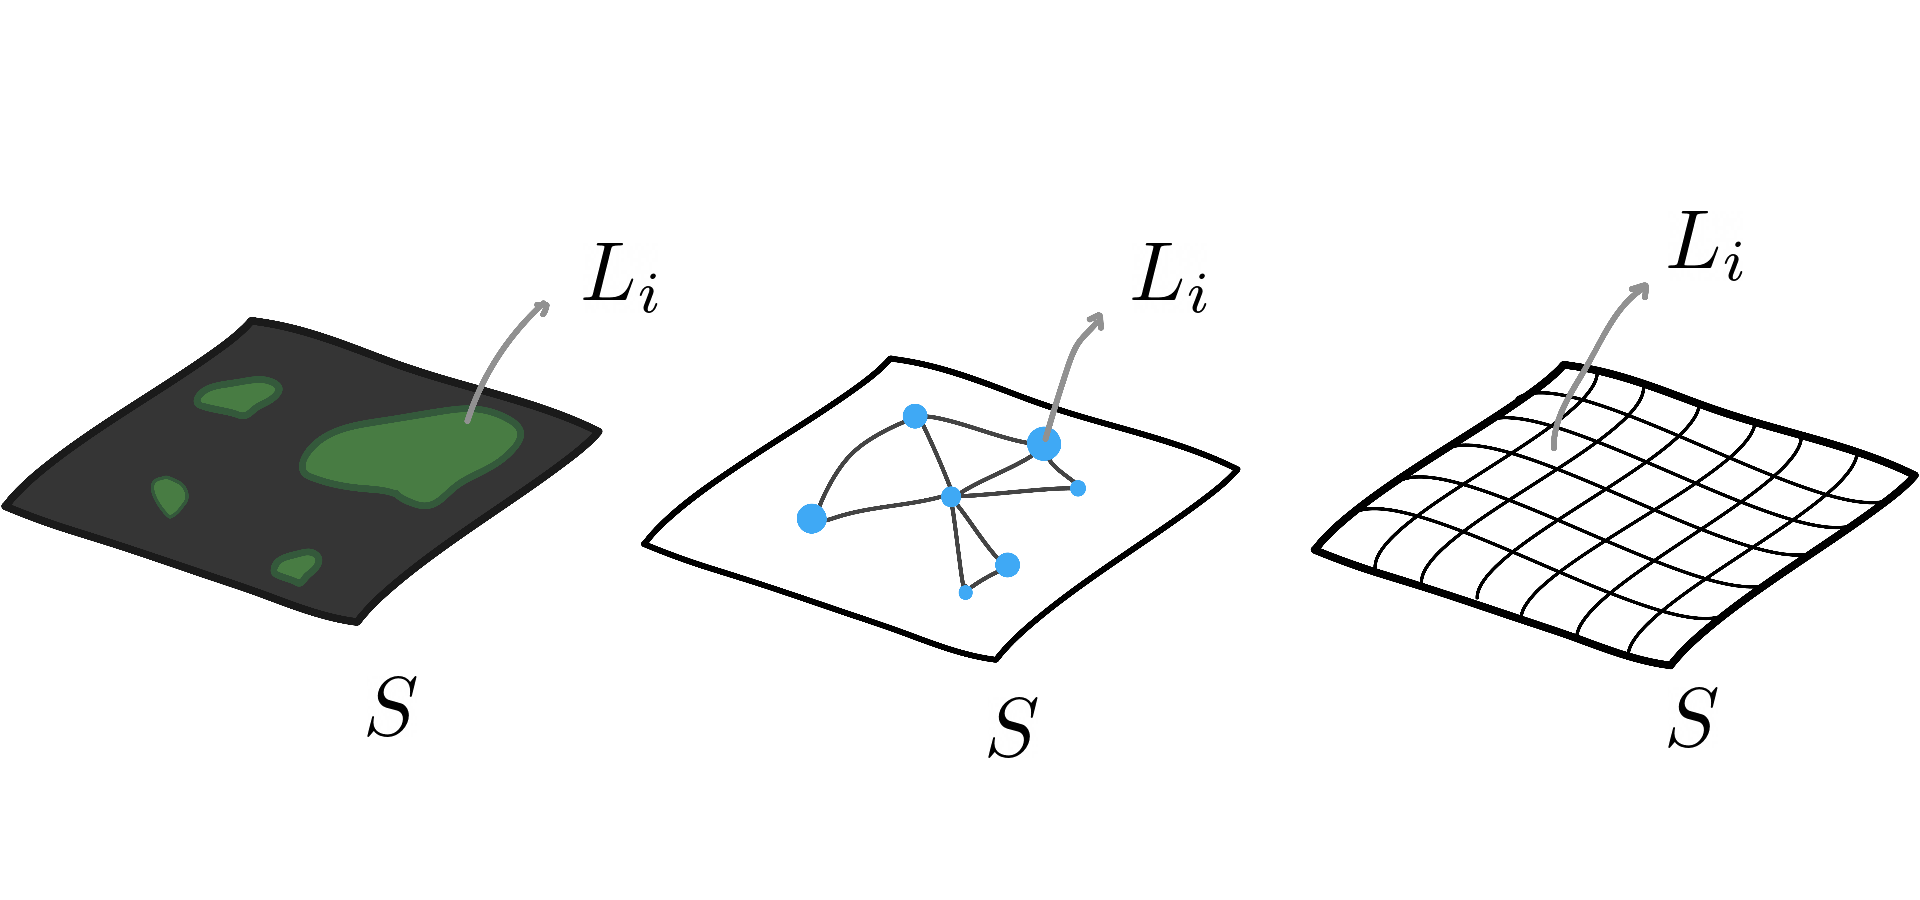
\includegraphics{/home/michael/prospectus/figures/different_spatial_models_w_labels.png}
  \caption{Three different representations of landscape structure often used in ecology (patches, spatial graph, lattice/raster). Each of these spatial models consist of discrete locations $L_i$ in a spatial domain $S$. Each $L_i$ interacts with $L_j$ according to the dispersal potential $\Phi$, see main text.}
  \label{fig:spatial_representations}
  \end{figure}

  \begin{figure}[H]
  \centering
  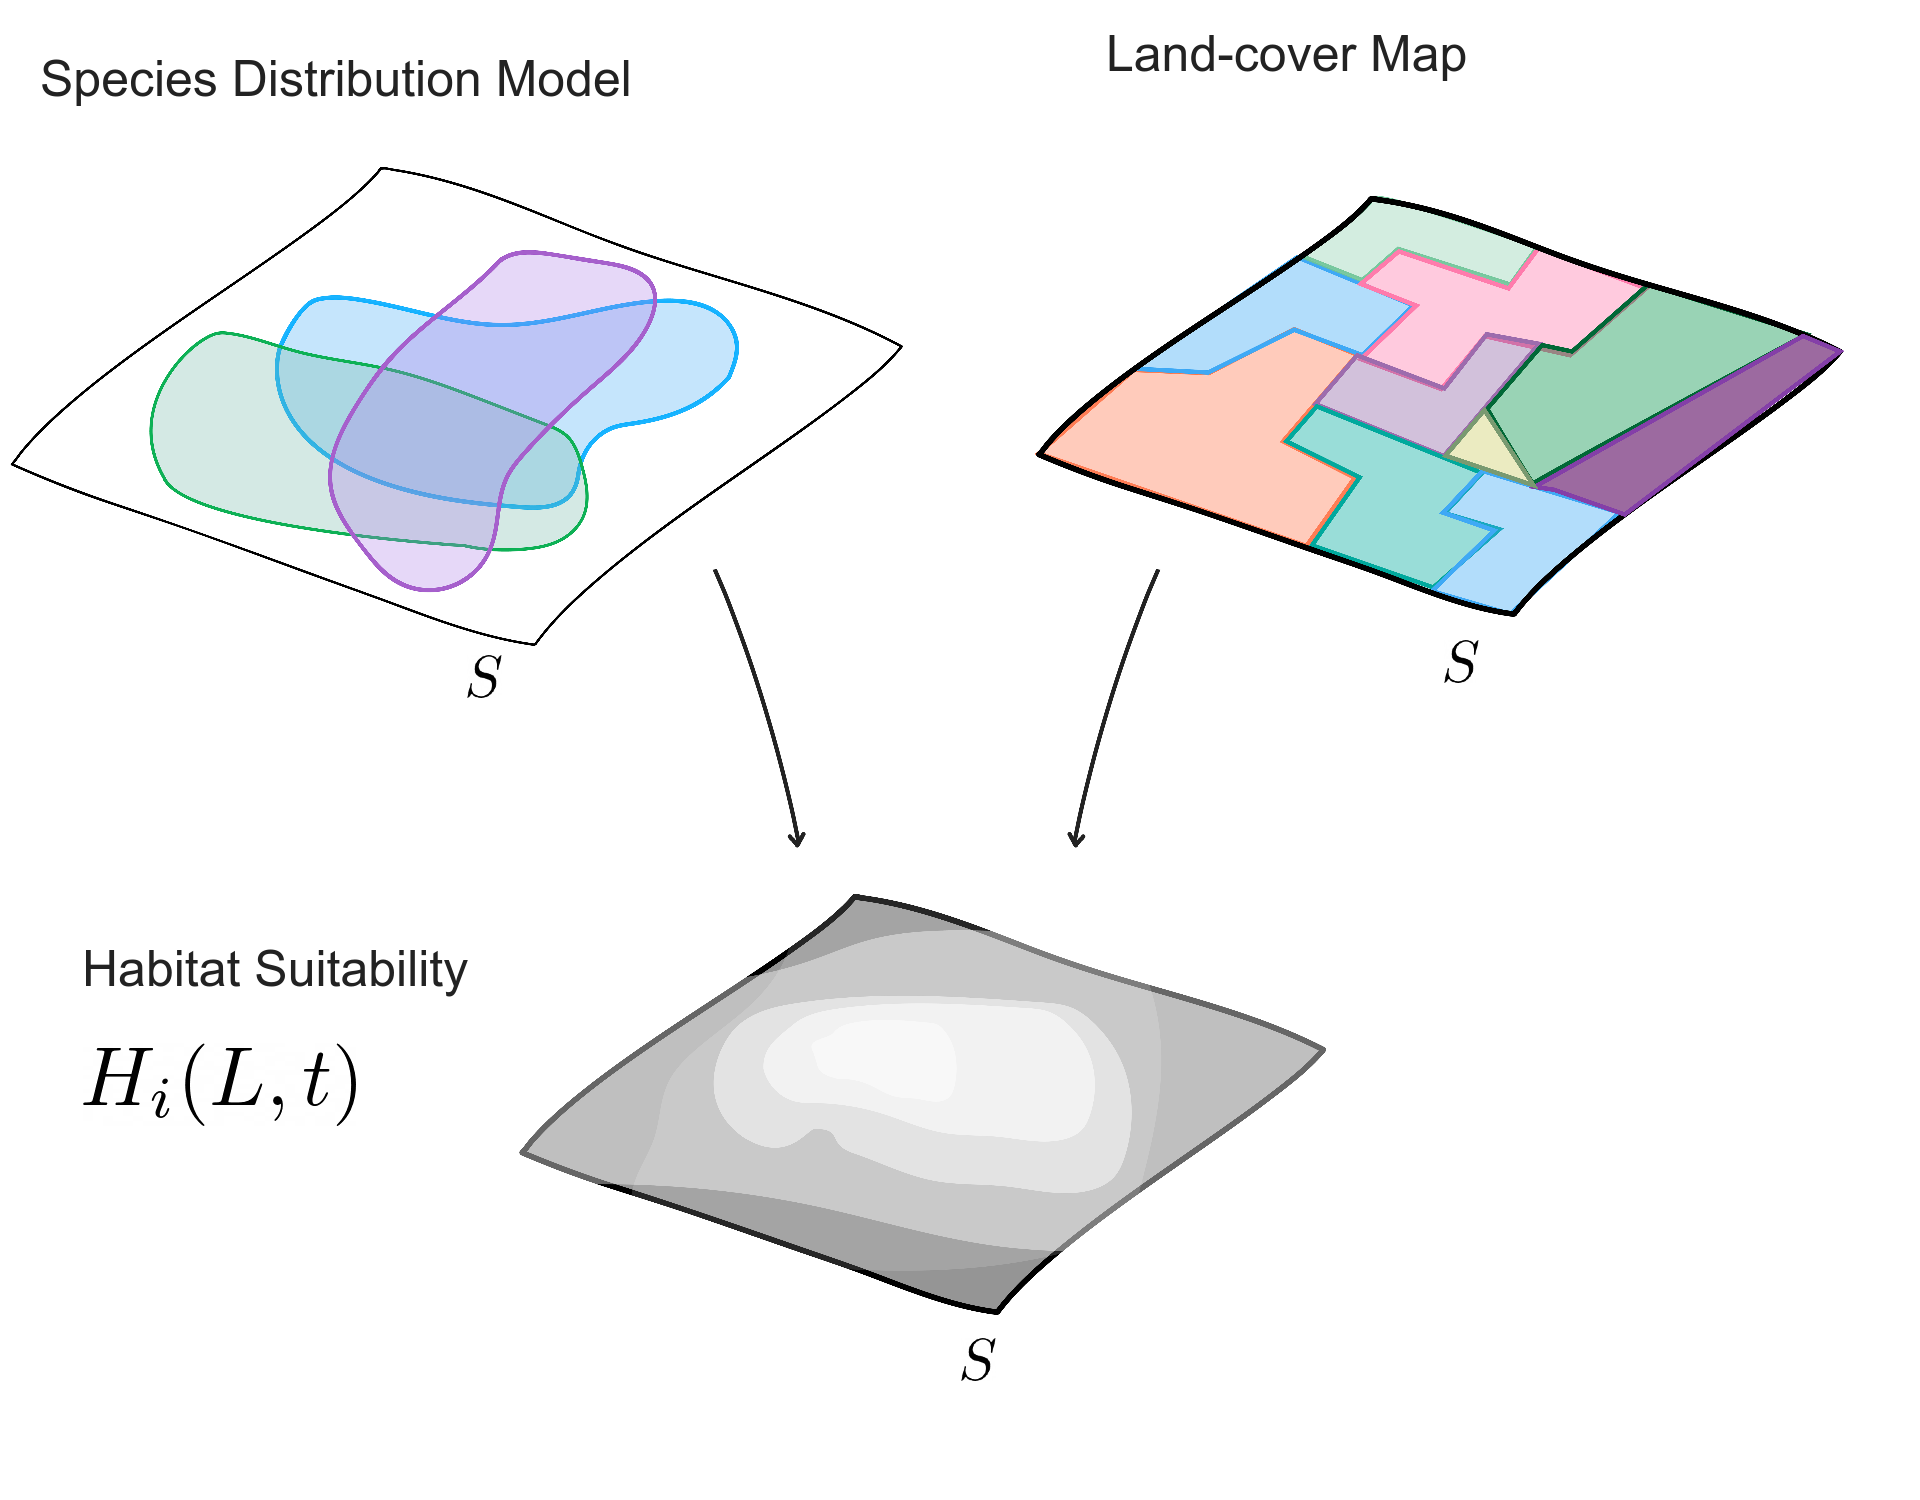
\includegraphics{/home/michael/prospectus/figures/habitat suitability w labels.png}
  \caption{Methods for creating a spatial model of habitat suitability for a species $j$. On large scales, habitat suitability is approximated by species distribution models. At smaller scales, land-use models and resistance surfaces.}
  \label{fig:habitat_suitability}
  \end{figure}
\item
  \textbf{Selection Model}: \(\{ E, T, \frac{\partial T}{\partial t}\}\)

  The selection model describes the traits \(T_i(L)\) of each species
  \(i\) at a location \(L\), and some function
  \(\frac{\partial T}{\partial t}\) which describes how \(T_i(L)\)
  changes over time as a function of both \(E(L)\) and \(T_i(L)\), which
  has several candidates from evolutionary biology
  \citep{price_selection_1970, queller_fundamental_2017}. Further, the selection model could include some measure of speciation based on differences in \(T_i\), however it
  doesn't directly relate to the questions in the proposed chapters, so we omit further details.
\item
  \textbf{Community Summary Model}: \(\{ C(\hat{B}) \}\)

  Finally, the Community Summary model is a summary statistic which maps
  from the observed state of biomass abundance (or occupancy)
  \(\hat{B}\) at some place and time to a value that represents
  community structure, e.g.~Shannon-entropy as a measure of
  \(\alpha\)-diversity. \(C\) could also be a measure of \(\beta\) or
  \(\gamma\)-diversity \cite{poisot_dissimilarity_2012}. However, if we are using a measure of
  \(\alpha\)-diversity or $\beta$-diversity,  we may need an additional summary statistic
  to encapsulate the distribution of \(C\) across all locations \(L\)---see Figure \ref{fig:metacommunity_space_w_distr}. One goal with the metacommunity model is to compare
  various metacommunity summary statistics to explore how they covary, and additionally if summary statistics are not differentiable even when the
  generative process is different.
\end{enumerate}

\begin{figure}[H]
\centering
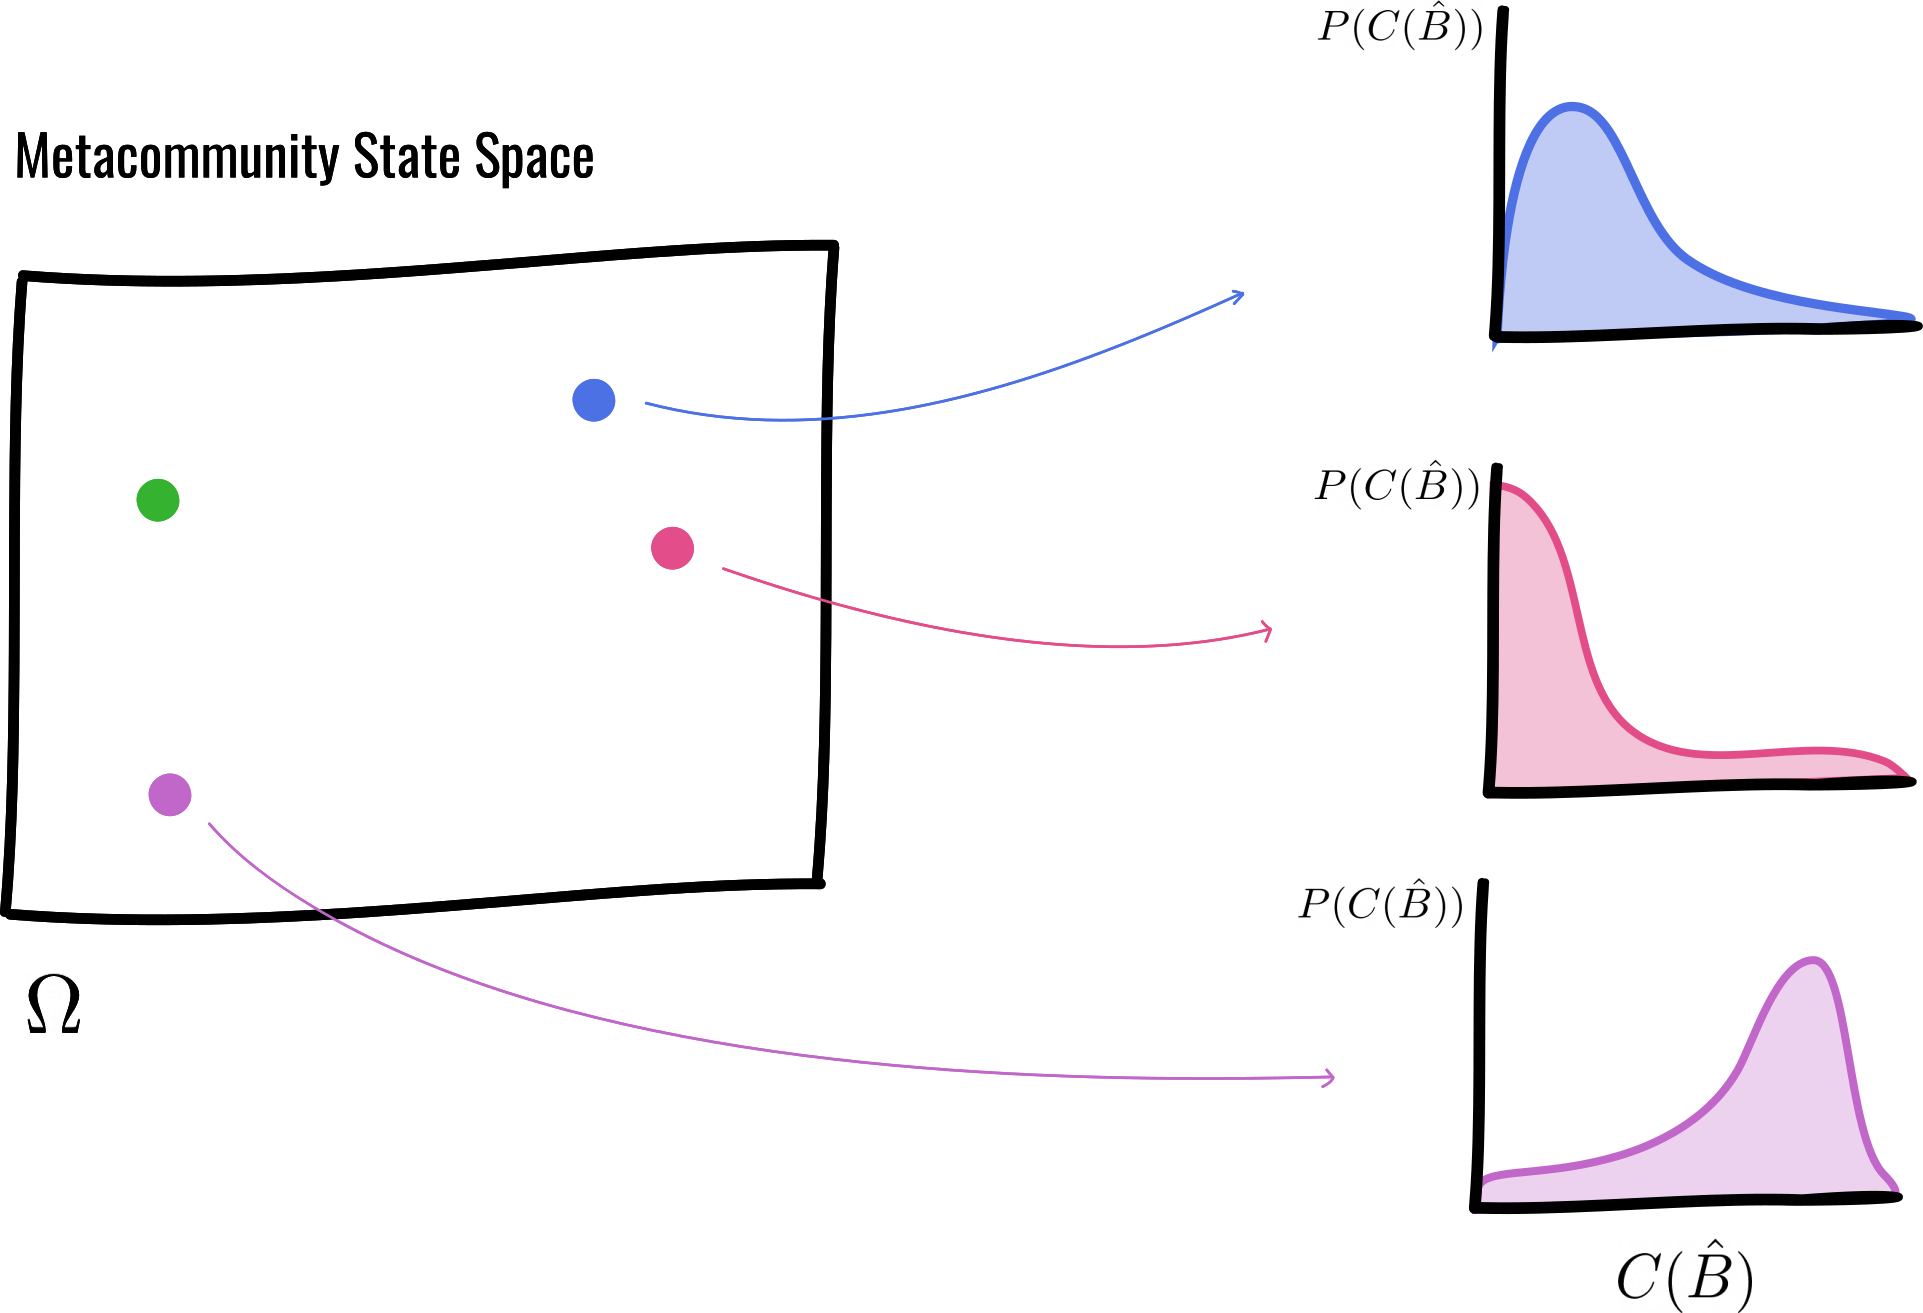
\includegraphics{/home/michael/prospectus/figures/metacomm_w_distributions.png}
\caption{Metacommunity state space $\Omega$ (left), as summarized by some statistic $C$. Each colored dot in $\Omega$ represents a different pseudoequilibria in state-space (unobservable to us), which corresponds with some value or distribution of values of the summary statistic $C(\hat{B})$. In the figure, each pseudoequilibrium corresponds with a distinct distribution of $\hat{B}$ (some measure of $\alpha$-diversity) across locations $L$ (right).}\label{fig:metacommunity_space_w_distr}
\end{figure}

% ________________________________________________________________________
%       section 3.3
%           software implementation
% ________________________________________________________________________
\hypertarget{software-implementation}{%
\subsection{Software Implementation}\label{software-implementation}}

Here, we describe how we will implement this metacommunity model as a
modular toolbox of software to simulate metacommunity dynamics that
interfaces with actual data and can be applied forecast in real systems.

\hypertarget{interfacing-with-generative-models-and-data}{%
\subsubsection{Building an Instance of the Model}
\label{interfacing-with-generative-models-and-data}}
In Figure \ref{fig:inputs} we can see how the conceptual objects in our metacommunity
model $A$ can interface with both generative models for the sake of using the
software as a ``virtual laboratory'' \citep{railsback_agent-based_2011} and
empirical data to forecast in real systems. The point is not necessarily
to vary all elements at once, but instead to have a modular set of tools
that cover a wide variety of use-cases. For example, if for a given use-case selection is not a relevant part of the question being asked, one could remove selection on traits from the model entirely.

\begin{figure}[H]
\centering
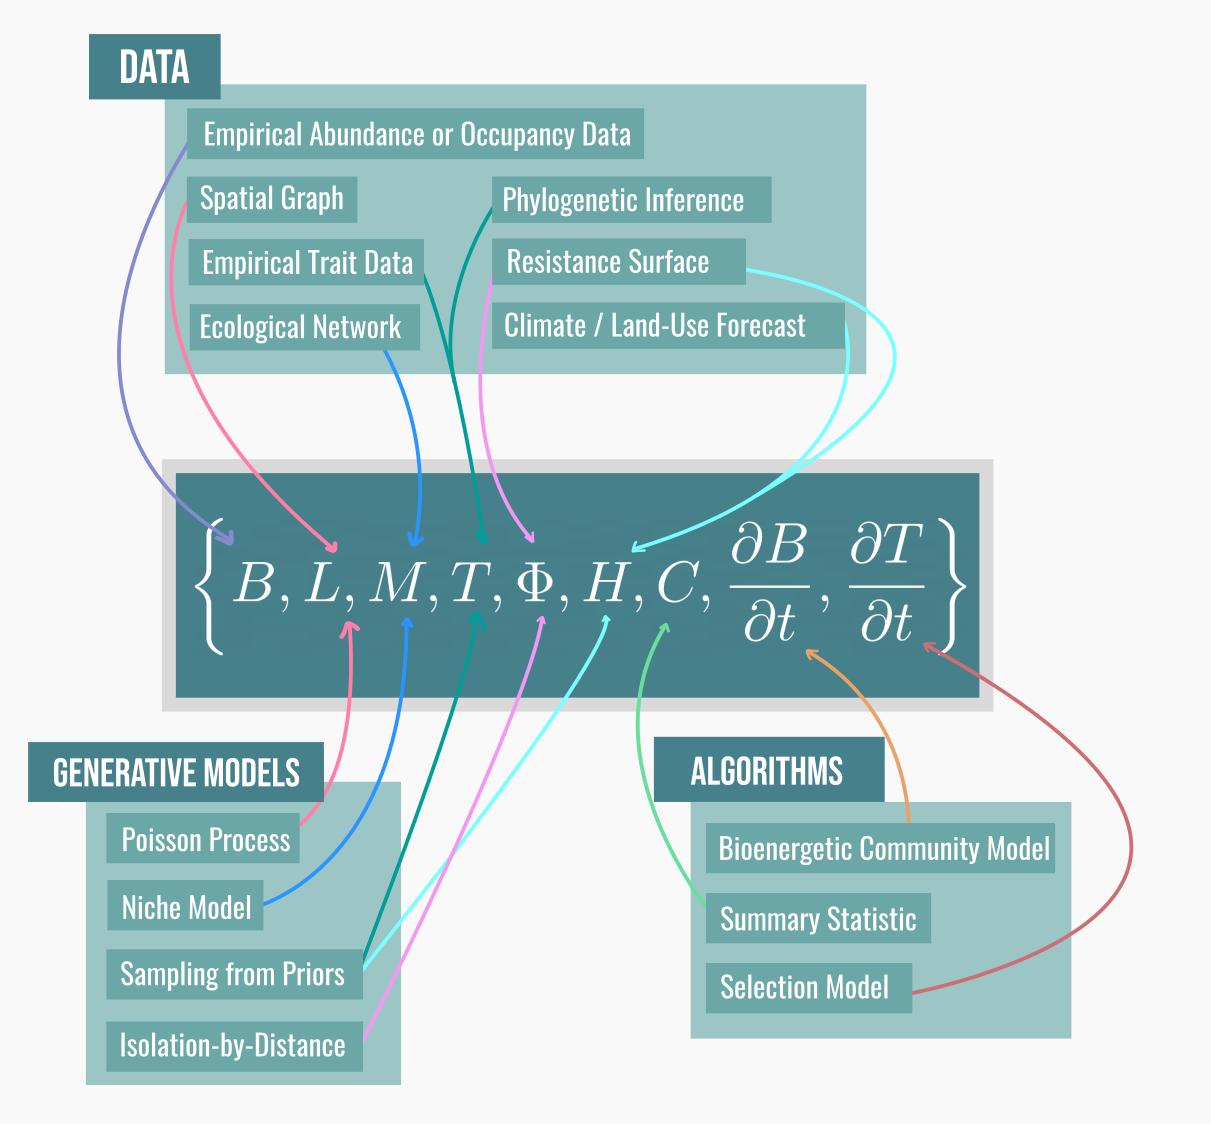
\includegraphics{/home/michael/prospectus/figures/inputs.png}
\caption{The way different elements of the model can interface with both empirical data (top) and generative models (bottom-left).} \label{fig:inputs}
\end{figure}

Every instance of a model $\hat{A}$ takes in parameters $\theta$ and inputs $\hat{x}$, and produces an outcome $y$. If we have observed $\hat{y}$, we can then use ABC methods to estimate $\theta$. For example, if the data we have are observed incidences of occupancy $\hat{y} = \hat{B}$, a metaweb $M$ and sampled environmental data $E(L)$, we can estimate the values of dispersal in $\Phi$ to determine if the metacommunity falls into the mass-effect or species-sorting paradigm. In this case, perhaps we would implement a simulation with and without trait variability, with and without stochastic dispersal, with different priors on $\Phi$, and so forth, fit each to the data, and use information criterion to determine which has the best predictive capacity via crossvalidation (see `Choosing Models and Priors` below).


\hypertarget{finding-the-pseudoequilibria-of-our-metacommunity-model}{%
\subsubsection{Describing Metacommunity Dynamics}
\label{finding-the-pseudoequilibria-of-our-metacommunity-model}}

For any given instance of a model $\hat{A}$, one can then simulate the dynamics of the community, at which point we have a sampled trajectory $B(t) \ \ \forall t \in \tau$ where $\tau$ is the simulation time domain. From this, we apply our summary statistic $C(B(t)) \ \ \forall t \in \tau$, and we have a trajectory in summary statistic space $\Omega$---see figure \ref{fig:density}. After running our model for many replicates, we can compute a density over the state-space $\Omega$ which represents the proportion of time the model spent in that part of $\Omega$.
One natural question is whether most models tend to converge to a small area of $\Omega$ and sit at equilibrium, or wander around state-space eternally.



\begin{figure}[H]
\centering
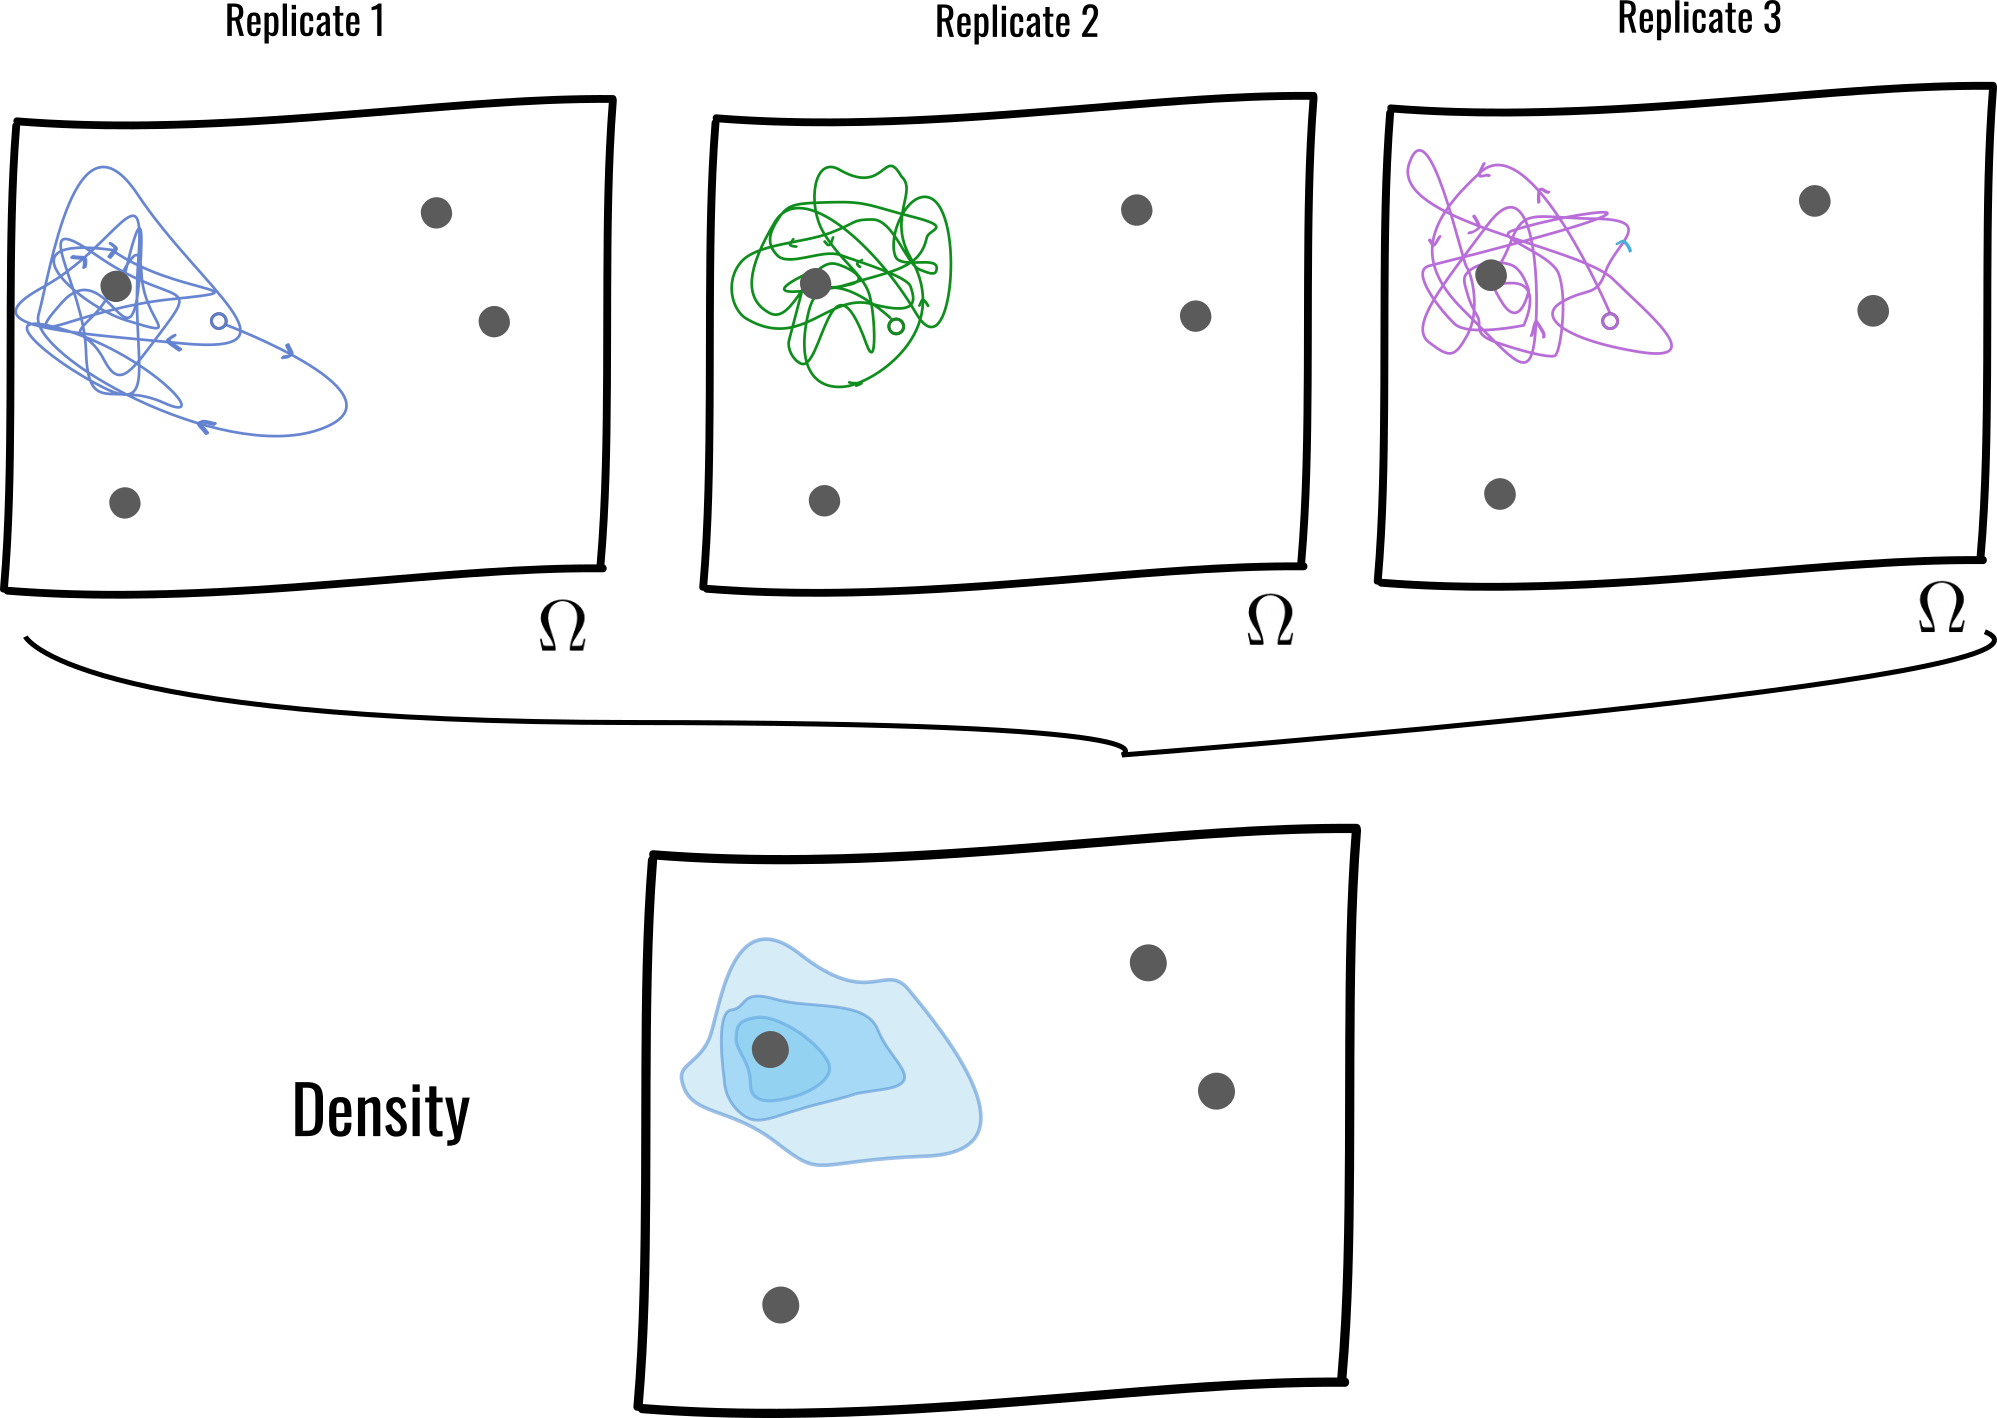
\includegraphics{/home/michael/prospectus/figures/density_plot.png}
\caption{A density over summary-statistic space $\Omega$, computer by averaging states across replicates. A density could be time-indexed, or averaged across all timesteps.} \label{fig:density}
\end{figure}

\hypertarget{fitting-to-data-with-abc}{%
\subsubsection{Fitting Simulations to Data with
ABC}\label{fitting-to-data-with-abc}}

In order to fit this metacommunity model to real data, we'll build an ABC sampler which takes in a definition of a simulation model $\hat{A}$
and a set of priors with hyperparameters
$\text{Priors}(\chi)$ as inputs, and estimates the posterior distribution---see Figure \ref{fig:abc}.

\begin{figure}[H]
\centering
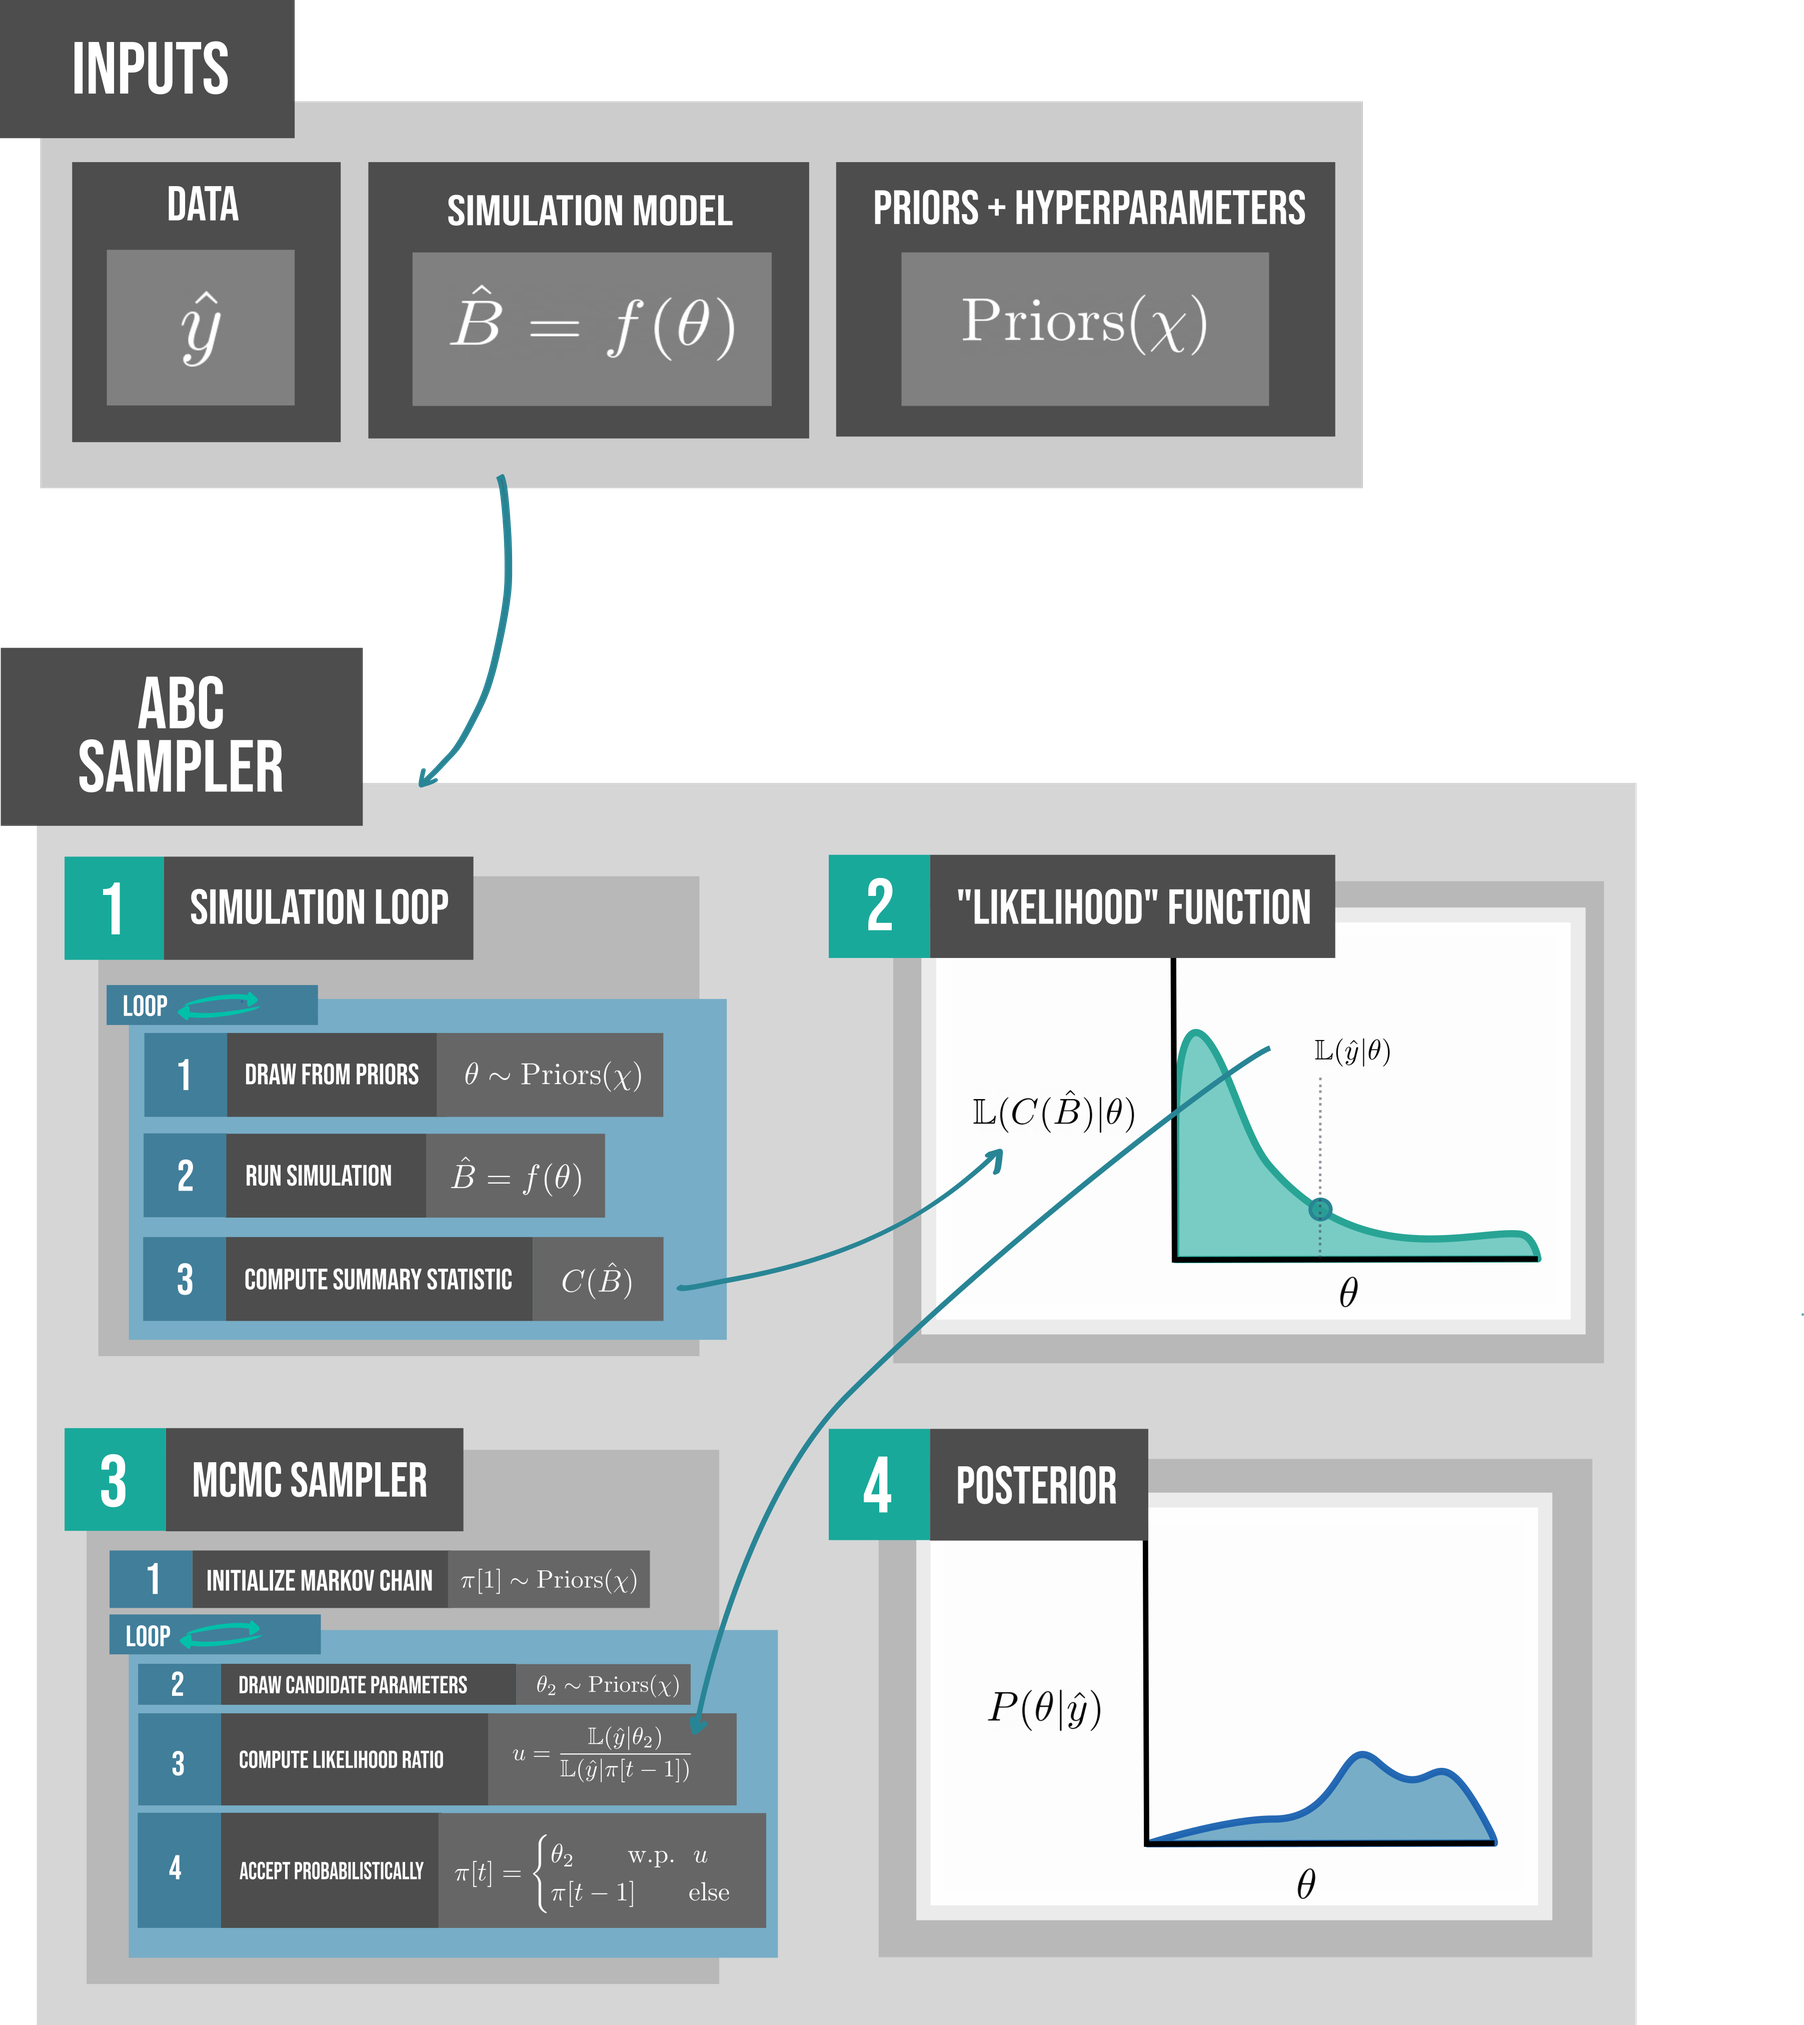
\includegraphics[height=12cm]{/home/michael/prospectus/figures/abc_conceputal.png}
\caption{ A conceptual overview of an Approximate Bayesian Computation (ABC) Sampler. An ABC Sampler takes in data $\hat{y}$, a simulation model $f(\theta)$, and a set of priors on simulation model parameters $\text{Priors}(\chi)$. The sampler generates an approximation of the likelihood function $\mathbb{L}$ by running a simulation loop (top-left), where each replicate the parameters $\theta$ are drawn from the priors. Need to fix the likelihood ratio in 3 to be multiplied by priors. As the number of replicates increases, the distribution of outcomes approaches the likelihood function  $\mathbb{L}(C(\hat{B}) | \theta)$ (top-right), which can be used to infer the posterior $P(\theta | \hat{y})$ via rejection sampling methods (bottom-left).  (This figure implies using a regression on simulation data in (2) to estimate $\mathbb{L}$, although early ABC papers use a tolerance around $L(\hat{y}|\theta))$ to do rejection sampling, see \cite{beaumont_approximate_2019})} \label{fig:abc}
\end{figure}


\hypertarget{choosing-models-and-priors}{%
\subsubsection{Choosing Models and Priors}\label{choosing-models-and-priors}}

If we have several competing simulation models or sets of hyperpriors, we can compare them using information criterion to see which one best describes the data--see Figure \ref{fig:info}.
To validate our models, we have few options beyond in-sample prediction. Crossvalidation methods typically repeatedly split the data into training sets $\{\hat{y}, \hat{x}\}$ and testing sets $\{\tilde{y}, \tilde{x}\}$. The model is fit on the training set, and then the predictive posterior derived from training data is used to predict $\tilde{y}$ given $\tilde{x}$. The goodness of fit on the model on the training set is quantified via some loss function, and then the overall models performance is summarized with some information criterion, often Cohen's $\kappa$.

\begin{figure}[H]
\centering
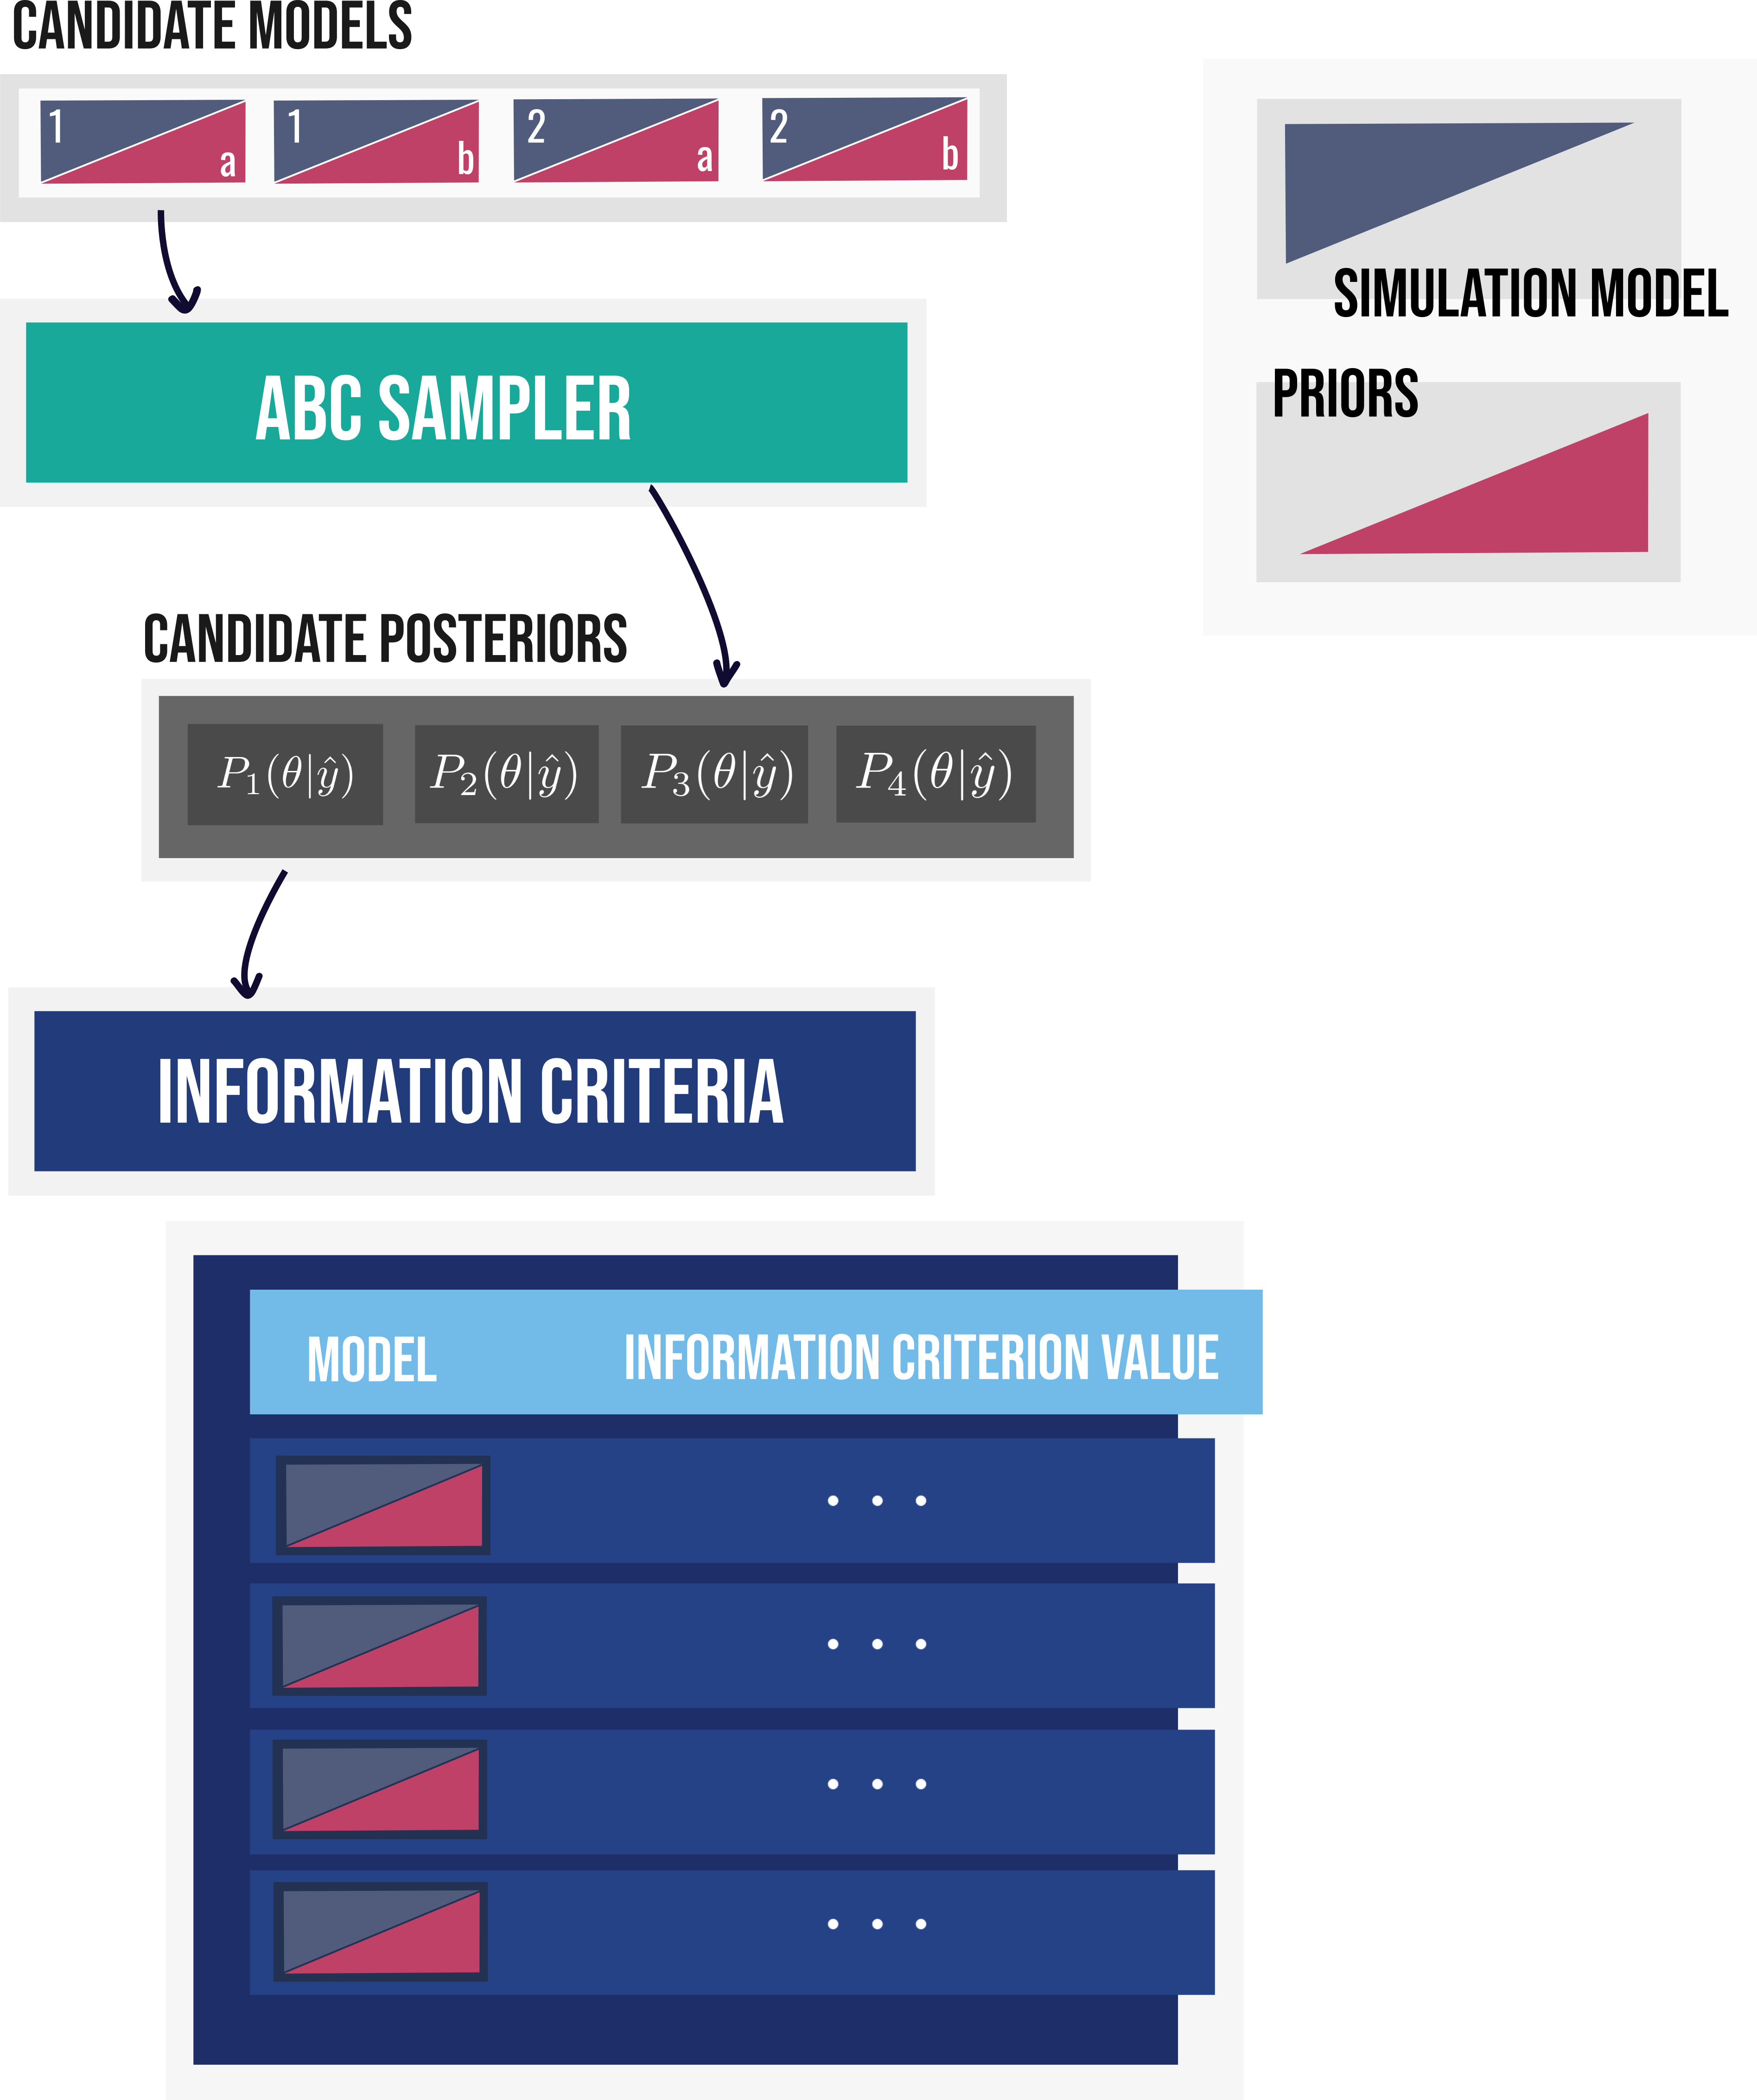
\includegraphics[height=12cm]{/home/michael/prospectus/figures/info_criteria.png}
\caption{The workflow for choosing a set of priors (red triange) and simulation models (blue triangles) for a given system. Run the ABC Sampler on each combination of priors and simulation models, and derive a candidate posterior distribution for each. Apply an information criterion (e.g. some type of crossvalidation) to determine which has the best predictive capacity on the data (see main text). Then the best models can then be used for forecasting. } \label{fig:info}
\end{figure}





\clearpage
\hypertarget{forecasting}{%
\subsubsection{Forecasting}\label{forecasting}}

Once we've estimated the best fitting posterior distribution $P(\theta | \hat{y})$, we can use it for forecasting via the best fitting simulation model. We can simply draw $\hat{\theta} \sim P(\theta | \hat{y})$ and run the dynamics model forward in time. Doing this many times, we get a density of predicted outcomes across the time domain $\tau$, with our uncertainty in parameter estimation propagated through to our forecast. If we have a forecasted model of land-use or climate change, we can also use that as an input into the model to shift $E_i(L, t)$ and $H_i(L,t)$ over time as well, while incorporating the uncertainty in those forecast models as well---see figure \ref{fig:forecasting}.

\begin{figure}[H]
\centering
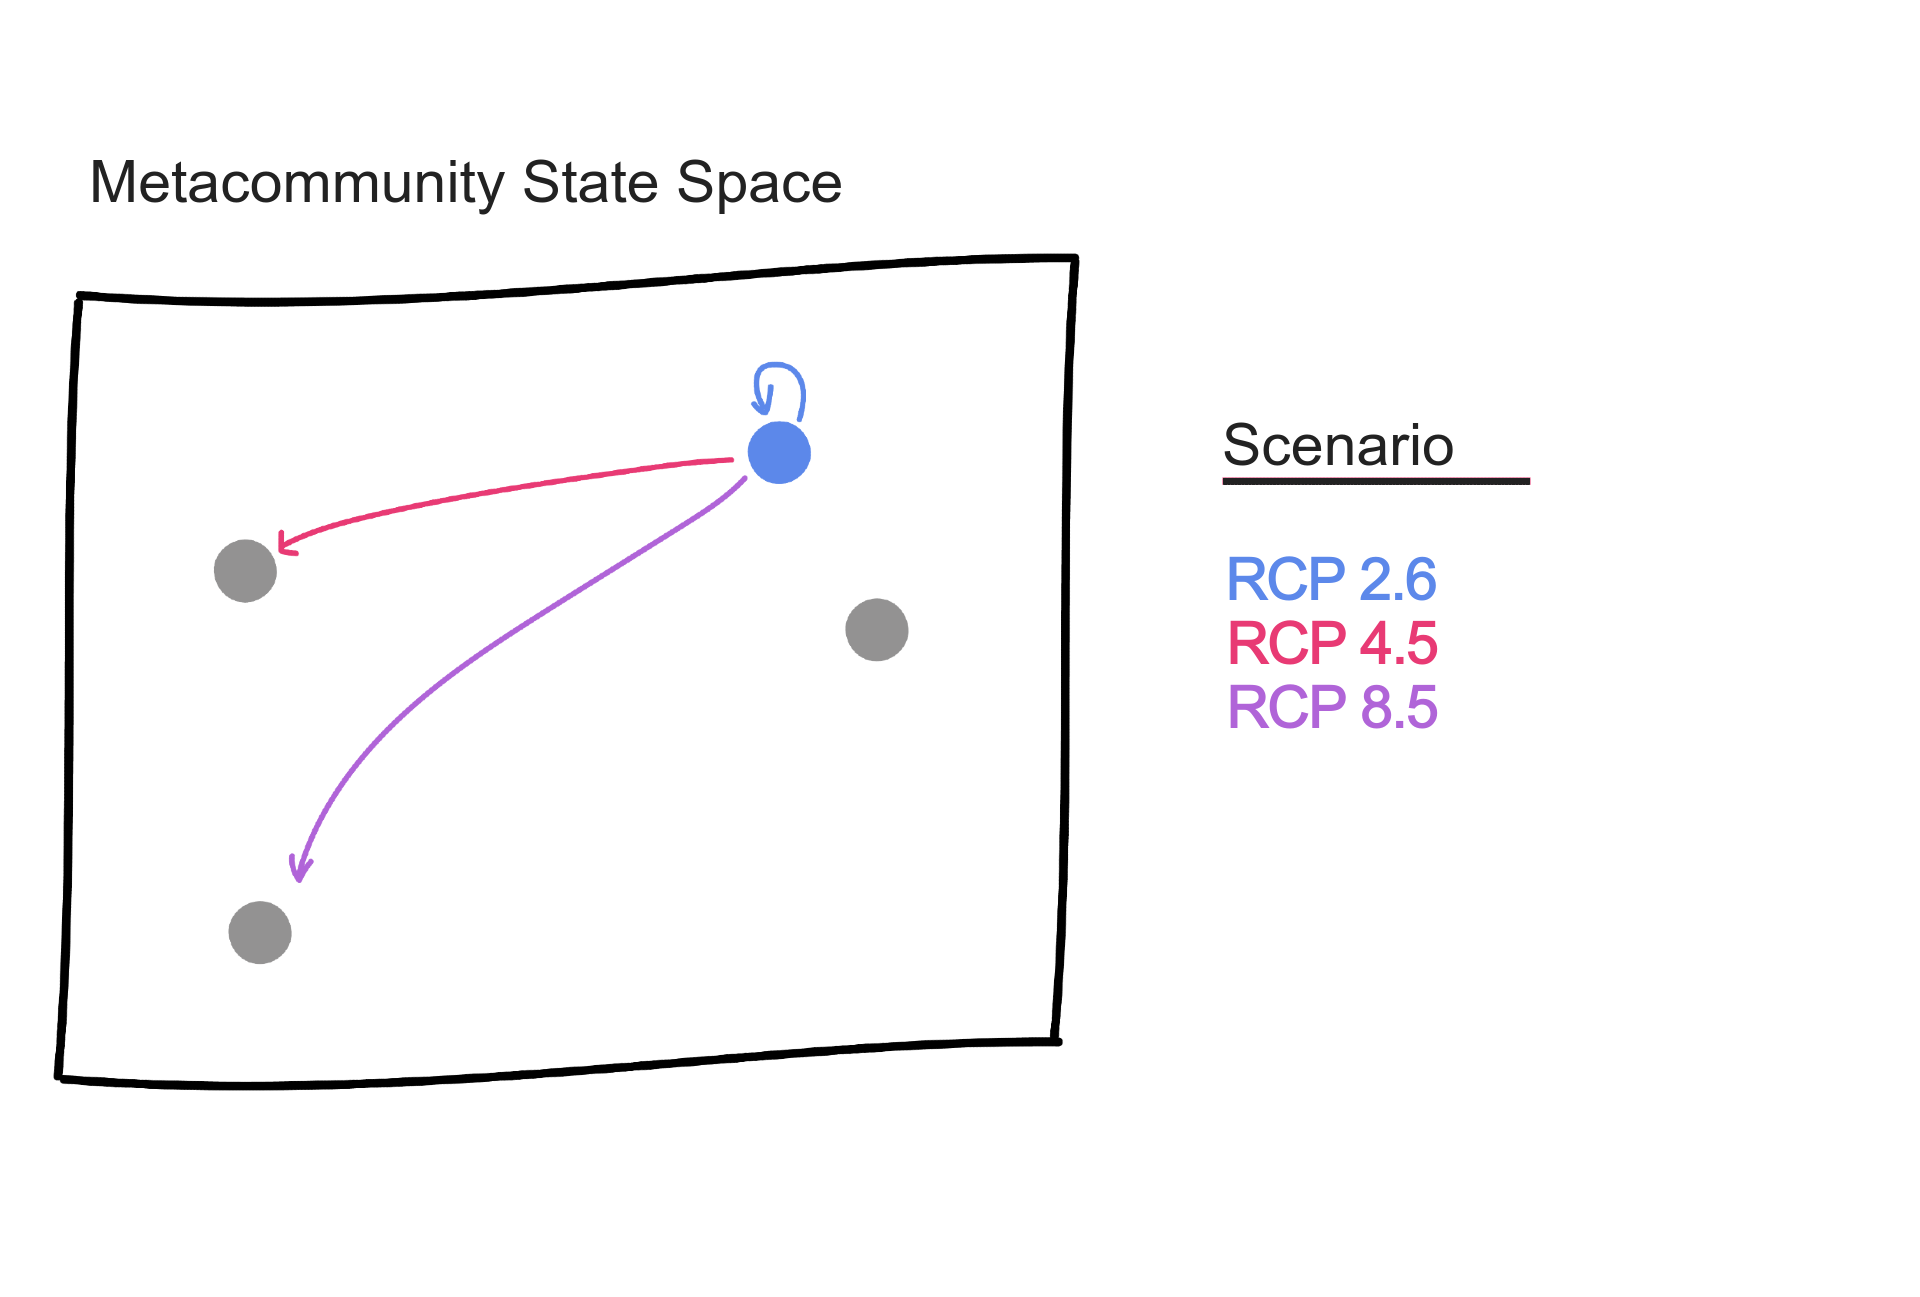
\includegraphics[height=12cm]{/home/michael/prospectus/figures/different_scenarios.png}
\caption{Top: forecasting the distibution of a metacommunity in state space $\omega$ under three different hypothetical corridor placements (represented as different colors). Bottom: the distribution of metacommunity state-space under hypothetical climate scenarios (colors). Grey dots in state space represent pseudoequilibria.} \label{fig:forecasting}
\end{figure}



% ________________________________________________________________________
%
%       CHAPTER 4
%
%           dissertation outline
%
% ________________________________________________________________________
\clearpage
\hypertarget{dissertation-outline}{%
\section{Dissertation Outline}\label{dissertation-outline}}

Here, we outline the general structure of the five planned dissertation chapters. At the moment, I'm planning for five chapters, the first being a review, the second being a software paper detailing the model, and then three research chapters where the model is applied. For the three research chapters, I'm planning to use the model as a ``virtual laboratory" in two of them, to first answer questions about metacommunity structure and diversity as a function of the different levels of Velland 2010's \citep{vellend_conceptual_2010} fundamental processes, and second to focus specifically on landscape connectivity's effects on diversity. In the final chapter, I aim to interface the model with data from a real system to forecast the effects of either climate or land-use change, depending on what data set will work best.

\subsection*{Chapter One --- Introduction and Review}

The opening chapter will be an introduction and review, which will look something like this document. The goal is to introduce the problems of understanding the processes behind metacommunity structure and dynamics, review (as opposed to overview) the literature in the adjacent fields, and summarize the major results of the dissertation.

\subsection*{Chapter Two --- Model Paper}

A chapter about the model, detailing the model as described above, how it is implemented as software, and how it can be used to answer questions in community ecology. This chapter would be aimed at a software journal, e.g. Methods in Ecology and Evolution. Hopefully we could use LEAP data as an empirical example in the actual paper for validation purposes, although that work might fall under chapter five in the dissertation.


\subsection*{Chapter Three  --- Metacommunity Assembly}

The third chapter will be use the model as a virtual laboratory to explore questions about why metacommunity structure varies in space and time. A list of major questions which I want to (at least partially) address:

\begin{itemize}
    \item At what proportions of selection, dispersal, and drift so we move in-between Leibold et al.'s four paradigms?
    \item At what spatial scales and temporal does community assembly shift from being driven by neutral to niche processes \cite{gravel_reconciling_2006} (see Figure \ref{fig:gonzalez2020}, borrowed from \cite{gonzalez_scaling-up_2020})?
    \item How does selection on biotic interactions (e.g. trait-matching) effect metacommunity structure and diversity?
    \item How does the dimensionality of trait-space effect the capacity for diversity in communities?
    \item What are different summary statistics used to measure $\alpha$, $\beta$, and $\gamma$-diversity in ecological networks, and how do they covary?
    \item When does environmental change cause metacommunity rewirings?
    \item What structural features do food-webs that stable under rewirings have in common? Do these predictions agree with our existing understanding of stability in food-webs     \cite{allesina_stability_2012}?

\end{itemize}

\subsection*{Chapter Four --- Space and Metacommunity Structure}
In the fourth chapter, I'm going to use the model as a virtual laboratory to determine the effects of landscape connectivity on metacommunity structure.

\begin{itemize}
    \item How does landscape connectivity change metacommunity structure and diversity capacity in a landscape?
    \item What makes a given metacommunity structure to sensitive to changes in landscape connectivity?
    \item Many previous models of metacommunity ecology assume equal dispersal capacity across species. What happens when we change this?
    \item Can we identify which habitat patches are most influential in allowing biodiversity to persist in a landscape?
    \item How does the spatial heterogeneity in the environment affect the diversity capacity of a landscape?
\end{itemize}
\begin{figure}[H]
\centering
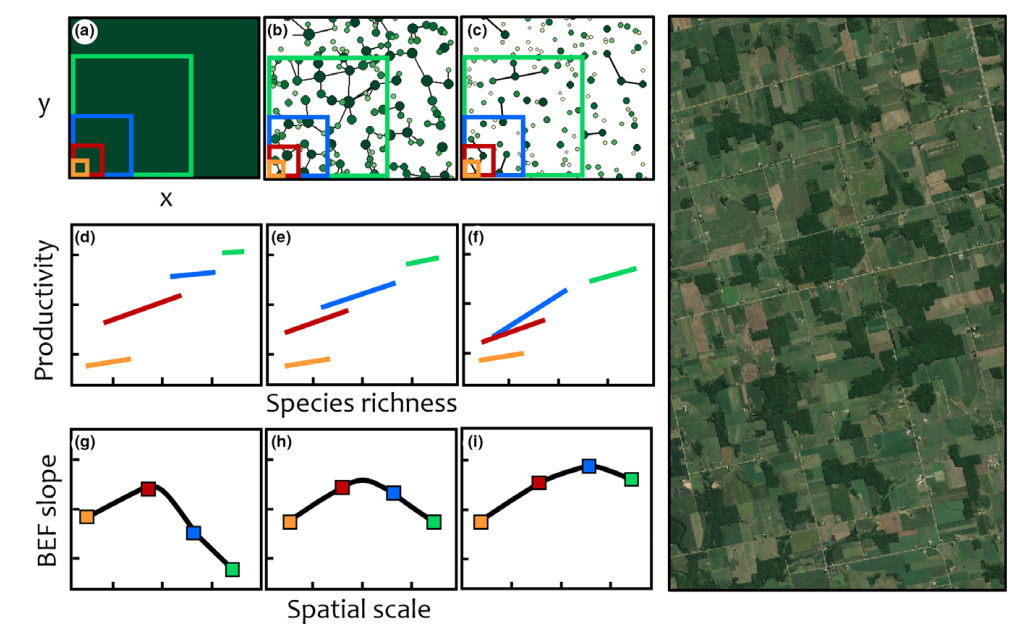
\includegraphics{/home/michael/prospectus/figures/gonzalez_ef_es.png}
\caption{From Gonzlez et al. 2020 \cite{gonzalez_scaling-up_2020}} \label{fig:gonzalez2020}
\end{figure}

\subsection*{Chapter Five --- Forecasting }

The fifth and final chapter will use the software's capacity cpaacities to interface with data to forecast in a real system. I need to get a better sense of what data is available here, but some options are:
\begin{itemize}
    \item A dataset with one metacommunity with temporal data --- LEAP, other experiments
    \item Use SDMs to forecast what rewirings of networks look like under different climate forecast models.
    \item Determine what effects corridors would have on community structure in a Protected Area
    forecast this local system in face of climate/land use, St. Lawrence region.
    \item Using the model with large dataset (like Mangal \cite{vissault_mangal_2019}) to see which processes are most likely driving each network, and to forecast community structure using whatever SDM/Habitat suitability models I can get for species in the dataset.
\end{itemize}




\hypertarget{conclusion}{%
\section{Conclusion}\label{conclusion}}

At this point, the next steps are to review the relevant literature that I've not yet seen---much of the purpose for reviewing the literature earlier was to determine find the gaps in what I've read. I'm also going to start building the software and looking into the data sources that are available. At this point, I'm most concerned about simulation time for these types of models getting computationally very expensive and slow. ABC requires many replicates to get a good description of the likelihood function, and doing crossvalidation requires fitting many times on subset of the data. Ideally fitting regressions to the likelihood function will speed this up and remain effective. Other concerns include if ABC is too sensitive to priors or typically provides results with poor fit. If so, parameter estimation for forecasting could be done using hierarchical models or something more well established in the literature.

% ________________________________________________________________________
%
%       REFERENCES
%
%
% ________________________________________________________________________
\clearpage
{
\footnotesize
\bibliography{refs}
}

\end{document}
